% \documentclass[sigconf]{acmart}
% 
% \usepackage{booktabs} % For formal tables
% \usepackage{color}
% \usepackage{textcomp}
% \usepackage{booktabs}
% \usepackage{graphicx}
% \usepackage{todonotes}
% \usepackage{multirow}
% \usepackage{adjustbox}
% \newcommand\mycheck[1]{\textcolor{red}{#1}}
% Copyright
%\setcopyright{none}
%\setcopyright{acmcopyright}
%\setcopyright{acmlicensed}
%\setcopyright{rightsretained}
%\setcopyright{usgov}
%\setcopyright{usgovmixed}
%\setcopyright{cagov}
%\setcopyright{cagovmixed}


% DOI
%\acmDOI{10.475/123_4}

% ISBN
%\acmISBN{123-4567-24-567/08/06}

%Conference
%\acmConference[WOODSTOCK'97]{ACM Woodstock conference}{July 1997}{El
%  Paso, Texas USA} 
%\acmYear{1997}
%\copyrightyear{2016}

%\acmPrice{15.00}


% \begin{document}
% \title{Influence of Reviewer Interaction Network on Long-term Citations: A Case Study of the Scientific Peer-Review System\\ of the Journal of High Energy Physics}
% % \titlenote{Produces the permission block, and
% %   copyright information}
% % \subtitle{Extended Abstract}
% % \subtitlenote{The full version of the author's guide is available as
% %   \texttt{acmart.pdf} document}
% 
% 
% \author{Sandipan Sikdar}
% %\authornote{Dr.~Trovato insisted his name be first.}
% %\orcid{1234-5678-9012}
% \affiliation{%
%   \institution{Indian Institute of Technology Kharagpur}
%   %\streetaddress{P.O. Box 1212}
%   \city{Kharagpur,India} 
%   %\state{Ohio} 
%   \postcode{721302}
% }
% \email{sandipansikdar@cse.iitkgp.ernet.in}
% 
% \author{Matteo Marsili}
% %\authornote{The secretary disavows any knowledge of this author's actions.}
% \affiliation{%
%   \institution{International Centre for Theoretical Physics}
%   %\streetaddress{P.O. Box 1212}
%   \city{Strada Costiera} 
%   %\state{Ohio} 
%   \postcode{34014 Trieste, Italy}
% }
% \email{marsili@ictp.it}
% 
% \author{Niloy Ganguly}
% %\authornote{This author is the
% %  one who did all the really hard work.}
% \affiliation{%
%   \institution{Indian Institute of Technology Kharagpur}
%   %\streetaddress{P.O. Box 1212}
%   \city{Kharagpur,India} 
%   %\state{Ohio} 
%   \postcode{721302}
%   }
% \email{niloy@cse.iitkgp.ernet.in}
% 
% \author{Animesh Mukherjee}
% \affiliation{
%   \institution{Indian Institute of Technology Kharagpur}
%   %\streetaddress{P.O. Box 1212}
%   \city{Kharagpur,India} 
%   %\state{Ohio} 
%   \postcode{721302}}
% \email{animeshm@cse.iitkgp.ernet.in}
% 
% 
% \renewcommand{\shortauthors}{Sikdar et al.}
% 
% 
% \begin{abstract}
% A `peer-review system' in the context of judging research contributions, is one of the prime steps undertaken to ensure the quality 
% of the submissions received; a significant portion of the publishing budget is spent towards successful completion of the peer-review by the publication houses. Nevertheless, the scientific community is largely reaching a consensus that peer-review system, although indispensable, is nonetheless flawed.
% A very pertinent question therefore is ``could this system be improved?". 
% In this paper, we attempt to present an answer to this question by considering a massive dataset of around $29k$ papers with roughly $70k$ distinct review reports together 
% consisting of $12m$ lines of review text from the Journal of High Energy Physics (JHEP) between 1997 and 2015. In specific, we introduce a novel \textit{reviewer-reviewer interaction network} (an edge exists between two reviewers if they were assigned by the same editor) and show that surprisingly the simple structural properties of this network such as degree, clustering coefficient, centrality (closeness, betweenness etc.) serve as strong predictors of the long-term citations (i.e., the overall scientific impact) of a submitted paper. These features, when plugged in a regression model, alone achieves a high $R^2$ of \textbf{0.79} and a low $RMSE$ of \textbf{0.496} in predicting the long-term citations. In addition, we also design a set of supporting features built from the basic characteristics of the submitted papers, the authors and the referees (e.g., the popularity of the submitting author, the acceptance rate history of a referee, the linguistic properties laden in the text of the review reports etc.), which further results in overall improvement with $R^2$ of \textbf{0.81} and $RMSE$ of \textbf{0.46}. Analysis of feature importance shows that the network features constitute the best predictors for this task.   
% Although we do not claim to provide a full-fledged reviewer recommendation system (that could potentially replace an editor), our method could be extremely useful in assisting the editors in deciding the acceptance or rejection of a paper, thereby, improving the effectiveness of the peer-review system. 
% 
% \end{abstract}
% 
% 
%   \begin{CCSXML}
% <ccs2012>
% <concept>
% <concept_id>10010405.10010476.10003392</concept_id>
% <concept_desc>Applied computing~Digital libraries and archives</concept_desc>
% <concept_significance>500</concept_significance>
% </concept>
% <concept>
% <concept_id>10003120.10003130.10011762</concept_id>
% <concept_desc>Human-centered computing~Empirical studies in collaborative and social computing</concept_desc>
% <concept_significance>300</concept_significance>
% </concept>
% </ccs2012>
% \end{CCSXML}
% 
% \ccsdesc[500]{Applied computing~Digital libraries and archives}
% 
% 
% \keywords{citations; reviewer-reviewer interaction network; prediction;}
% 
% 
% \maketitle
% 
% %\vspace{-3mm}

\section{Introduction}

%\begin{enumerate}
%\item Although there are many existing graph sampling algorithms not all properties are represented correctly in the obtained sample. For example random not sampling is able to mimic the degree distribution of the original graph but fails to retain the clustering coefficient. We hence propose that separate sampling strategies should be designed in order to retain a specific property in the sample. We consider community structure i.e., we develop a sampling algorithm which retains the community structure of the original graph. The motivation behind such a algorithm is that generally community detection algorithm are generally computationally expensive and a sample which retains the community structure of the original graph would allow for running community detection algorithms on it and then extend it to the large graph thereby saving computing resources. It would be particularly helpful in cases where it is not known beforehand which community detection algorithm to use and hence all of them need to be executed in order to obtain the best result. One can run all the algorithms on the sample and decide on using a particular algorithm.

%\item As mentioned earlier community detection algorithms are computationally expensive and hence running them on large graphs could be very expensive. Our algorithm is designed in such a way that community detection algorithm is executed on a small scale and then community of a new node is decided incrementally. We thereby obtain a representative cluster structure which is computationally much less expensive. 
%\end{enumerate}
\if{0}
Sampling has been a fundamental part of statistics in is widely used in cases where it is difficult to perform analysis on the whole population. With proliferation of large scale graph data it is often required to measure properties of a large graph which are computationally very expensive. An obvious solution is to obtain a smaller representative sample of the graph and measure its properties assuming that the result would be similar to the original. But how to obtain a good representative sample? The question was first proposed in \cite{leskovec2006sampling} and the researchers have subsequently come up with several sampling algorithms \cite{ahmed2010reconsidering,maiya2010sampling,rasti2009respondent,ribeiro2010estimating}. Most of these works are mainly aimed at preserving specific graph properties. In \cite{maiya2010sampling} the authors argue that it is difficult to obtain a universally representative sample which preserves all the graph properties. 

Another interesting observation is that most of the real-world graphs evolve over time with new nodes and edges being added to the graph. Such graphs are represented through a streaming graph model whereby the 
\fi


Nowadays graphs are so large that their analysis in entirety can be intractable and impractical. How then one should proceed in analyzing and mining these graphs? Traditional approaches include designing more efficient algorithms or leveraging computing power through parallelization or distributed computing. Unfortunately, these existing methods are not always easily available as an option. Another approach that has received recent attention is the technique of {\em sampling}~\cite{leskovec2006sampling}.

Although data sampling is exhaustively studied in statistics~\cite{doucet2000sequential,hastings1970monte}, sampling from graphs has got only limited attention~\cite{gjoka2010walking,maiya2010sampling,rasti2009respondent,ribeiro2010estimating}. Moreover, when it comes to the case of sampling from {\em streaming graphs} (where edges arrive in discrete time intervals) there is hardly any work beside~\cite{aggarwal2011outlier,ahmed2014network}. 
Existing graph sampling methods are mostly designed for {\em static graphs} and aim at preserving general structural properties (such as degree distribution, clustering coefficient etc.) of the original graph in the sample. However we posit that it is impossible for any sampling method to produce a universal representation that can preserve {\em all} sorts of graph properties of the original graph; rather graph sampling should be {\em application specific}. For instance, sampling method designed for information diffusion should preserve the hubs (high-degree nodes) in the sample; whereas sampling for outbreak detection (such as disease outbreak) should preserve the nodes with high local clustering coefficient.

In this work, we propose a novel sampling algorithm that preserves the original {\em community structure}\footnote{In this work, we consider disjoint community structure.}. A community in a graph
is a cluster of nodes more densely connected among themselves than to others \cite{wasserman1994social}. Identifying community structure is important, as they represent the {\em mesoscopic view} of the graph and often correspond to real social groups, functional groups, or demographic similarity etc.~\cite{girvan2002community}. The ability to easily construct a sample consisting of members from diverse communities has several important applications. For instance, in marketing, surveys often seek to construct stratified
samples that collectively represent the diversity of the population \cite{Kolaczyk:2009}. Many popular community detection algorithms considered to be accurate are also computationally expensive~\cite{danon2005comparing,fortunato2010community}. Representative graph sampling, then, provides a potential solution for inferring and approximating global, latent properties such as these in large graphs. By sampling a representative subgraph, analysis can be performed on the sample instead of the larger graph. Results could, then, be generalized
to the larger population, which, in this case, is the original graph. However, if one still intends to run an accurate and computationally-expensive community detection algorithm on large graphs
and is confused which one algorithm to choose, she can run several potential algorithms on the sample graph and choose one that performs best. Then that algorithm can be used to detect communities from the original large graph.

{\bf Our contributions:} We propose~\compas, a novel sampling algorithm on streaming graph (most realistic graph representation \cite{aggarwal2011outlier,ahmed2014network}) that is capable of
representing and inferring community structure in the original graph. \compas~systematically interweaves graph sampling and community detection so that one gets benefits from the other to produce a more representative sample. In particular, our contributions are three-fold:
\begin{itemize}
\item To our knowledge \compas~is the first {\em community-preserving} sampling method for {\em streaming graphs}. Along with the sample, \compas~also produces the community structure of the sample.

\item Empirical evidences on synthetic graph and different real-world graph demonstrate that the sample generated by \compas~is not only the most representative to preserve the community structure, but also is quite competitive in reproducing the other general graph properties. %\TODO{Report numbers here. For instance, our results are x\% better in preserving the community structure compared to the most competitive baseline. Similarly report for other properties.}
The average performance of our algorithm reaches 85.5\% of the most informed algorithm (GA \cite{tong2016novel}) on static graphs.

\item We show additional benefits of \compas~through two applications -- (i) selection of right community detection algorithm for large graphs, and
%(ii) message spreading in streaming graph, 
(ii) selection of (limited) training set for online learning. We obtain a performance that is within 95.6\% and 90.5\% of the most informed algorithm (i.e., GA) available for static graphs for first and second applications respectively.
%\TODO{Are the benefits compared to some baselines? Then again report improvements here.}
\end{itemize}










% \vspace{-4mm}


\noindent
\section{Reviewer-reviewer interaction network}
\label{rev_int_net}
In this section, we construct a reviewer-reviewer interaction network and show that its properties are linked to the future scientific impact of a paper (measured in terms of the cumulative citation count). In specific, we find that the position of the assigned reviewer in the network (measured in terms of degree, centrality, clustering coefficient and PageRank) could be used to predict the long term citation of the paper. 
 
The reviewer-reviewer interaction network is created with each node representing a reviewer and an edge exists between two reviewers if they have been assigned by at least one common editor. We devote the rest of the section in demonstrating the importance of the various structural properties of the network in determining the long term citation of the paper. Note that there are 4035 unique reviewers in the system each of which form a node in this network.

\begin{figure*}
\centering
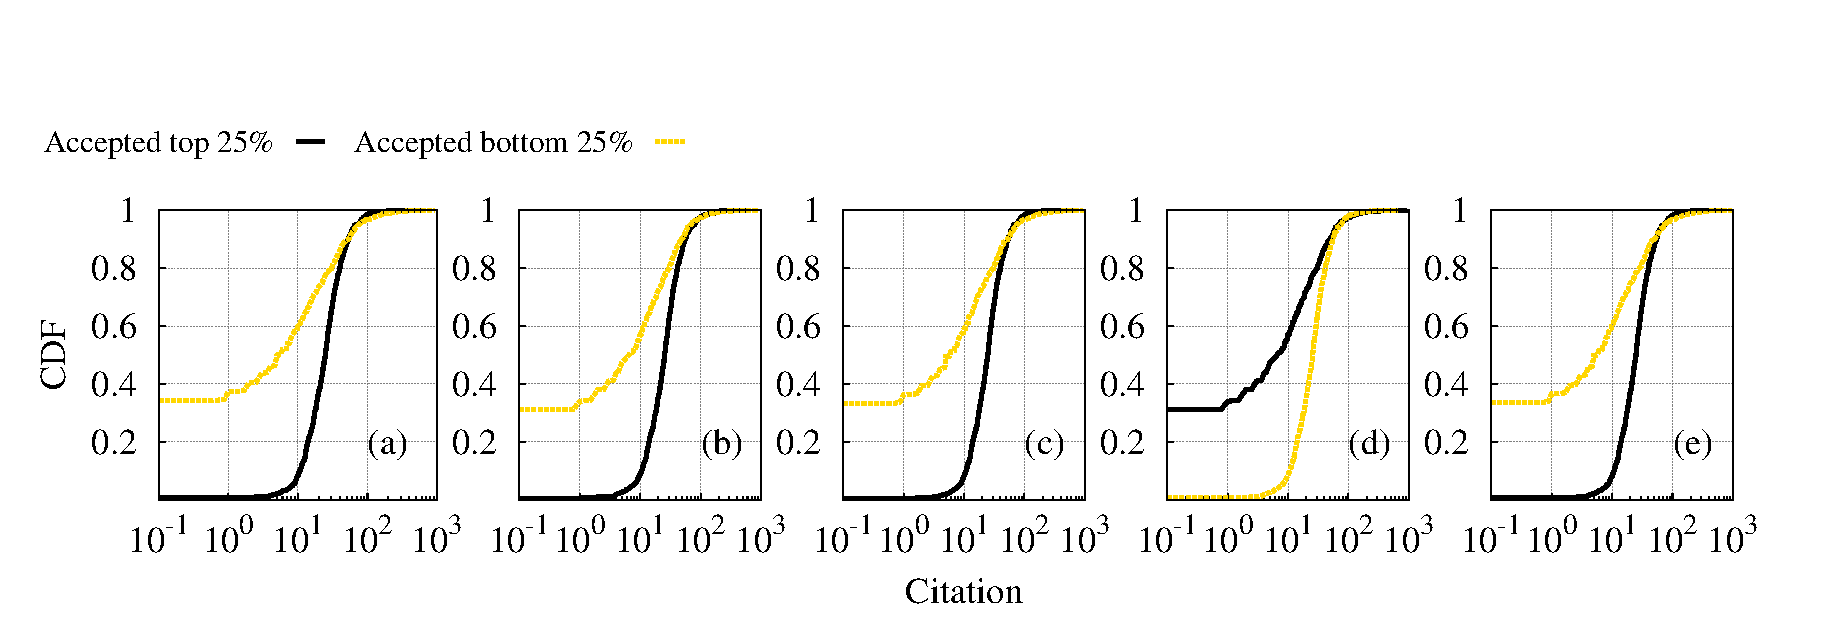
\includegraphics[width = 0.95\textwidth]{figures/citation_.eps} 
\caption{\label{fig:net_citation} Cumulative distribution function (CDF) of citations received by the papers (accepted) reviewed by referees in top 25\% and bottom 25\% reviewers ranked according to (a) degree, (b) betweenness centrality, (c) closeness centrality (d) clustering coefficient values and (e) PageRank in the reviewer-reviewer interaction network.}
\end{figure*}

\subsection{Degree (Deg)}
Degree of a node $v$ is the number of other nodes it is connected to in the network. A node with a higher degree in the reviewer-reviewer interaction network would indicate (i) assignment from multiple editors, (ii) assignment from a reputed editor (with large number of assignments) which in turn would indicate the reputation of the reviewer. To verify our hypothesis, we rank the reviewers based on their degree in the network and calculate the mean citation of the papers reviewed by the reviewers in the top and the bottom 25\% of the rank list. We observe that  the papers reviewed by the top 25\% reviewers receive much higher citations than the those reviewed by the bottom 25\% reviewers (refer to fig.~\ref{fig:net_citation}(a)).    

\subsection{Betweenness centrality (BC)}

Betweenness centrality of a node quantifies the position of a node based on the number of shortest paths the node is part of. For every  pair of nodes in the network there exists a shortest path between them. Betweenness centrality of a node ($v$) is the fraction of all such paths that pass through $v$. In the reviewer-reviewer interaction network, a high  centrality value would indicate assignment by multiple editors and that this node acts as a bridge between them. We again rank the reviewers based on the betweenness centrality values and calculate the average citation of the papers. We find that the papers accepted by the top 25\% reviewers tend to be cited more compared to those accepted by the bottom 25\% (refer to fig.~\ref{fig:net_citation}(b)). 

\subsection{Closeness centrality (CC)}

Formally closeness centrality of a node in a network is the inverse of the sum of length of its shortest path to all other nodes in the network. Hence higher centrality value indicates that the node is more closer to all other nodes in the network. In the reviewer-reviewer interaction network, a reputed reviewer will be assigned by multiple reviewers and hence will be closer to the other reviewers in the network. This is represented in fig.~\ref{fig:net_citation}(c), where we show that the papers accepted by top 25\% most central reviewers 
are cited more often compared to the bottom 25\% reviewers. 

\subsection{Clustering coefficient (Clus)}

Clustering coefficient of a node is measured as the fraction of connections among the neighbors of the node. For the reviewer-reviewer interaction network, every reviewer assigned by a common editor is connected to every other reviewer in the network. A reviewer assigned by many editors would actually act as a bridge between two cliques and hence would have a lower clustering coefficient value compared to a reviewer who is part of a single clique (always assigned by a single editor). This is further demonstrated in  fig.~\ref{fig:net_citation}(d) where we observe that the papers accepted by reviewers having lower clustering coefficient tend to be cited more.

\subsection{PageRank (PR)}

PageRank is a link analysis based algorithm that calculates for each node its relative importance within 
the network. Specifically, PageRank outputs a probability distribution which is used as the likelihood of a random walker to end up in a specific node. We simulate PageRank on the reviewer-reviewer interaction 
network to obtain the relative importance of each node. Further analysis indicates that the papers accepted by the top 25\% reviewers (based on PageRank) are cited more often compared to those accepted by the bottom 25\% reviewers (refer to fig.~\ref{fig:net_citation}(e)). 

The above results thus indicate that simple network properties of the reviewer-reviewer interaction network could be highly effective in predicting the long-term citation of the paper at the time of publishing. 
\medskip


\noindent
\subsection{Supporting features}
Most of the works~\cite{yan2012better,chakraborty2014towards} related to predicting long-term citation of papers considers a wide set of author related features, papers-centric features and citation pattern of the paper in the first few years from the date of its publication. 
Further, our dataset allows us (unlike the existing datasets) to look into several other features related to the review-process like the review report, the behavior of the assigned referee, the number of rounds of reviews the paper went through and others. 
We consider the above features as well as those existing in the previous literature (wherever available) as the set of supporting features. The features are categorized into (i) paper based, (ii) review report based, (iii) author based and (iv) reviewer based. Apart from investigating the effectiveness of a feature in determining the long-term citation of the paper, we also point out some interesting observations that we could make while analyzing the dataset.    

\subsubsection{Paper based features}
\label{analysis}
We have already observed that the average number of citations received by accepted papers is 31.80; for rejected papers the corresponding value is 9.45 (refer to table~\ref{tab1}). Note that for each paper we consider the citations accrued by it till 2015 from the date of publication.
We further consider all the accepted and the rejected papers and segregate them based on the number of citations received. We consider different citation buckets and plot the fraction of accepted and rejected papers in each of these buckets in figure~\ref{fig4} {\bf (Left)}. Note that the bucket sizes are in increasing powers of 2. Typically, the buckets are $\leq 1$, $2$, $(>2$ and $\leq 4)$ and so on. It can be clearly observed that accepted papers are cited more often compared to the rejected ones. Nevertheless, on further analysis we find that there could be a few exception cases where the rejected paper could make a place in higher impact journals (compared to JHEP) and, eventually, receive a high volume of citations in future. We present two such pathological cases below -- {\bf Case 1:} Rejected after two rounds of review, later accepted at Physics Letters B, citations: 1209; {\bf Case 2:} Rejected after one round of review, later accepted at Computer Physics Communications, citations: 929. We perform a thorough analysis of these irregular cases later in the paper.



\subsubsection*{Number of review rounds (RR)}

 \begin{figure*}[htpb]
 \centering
 %\vspace{-4mm}
 \begin{tabular}{ccc}
 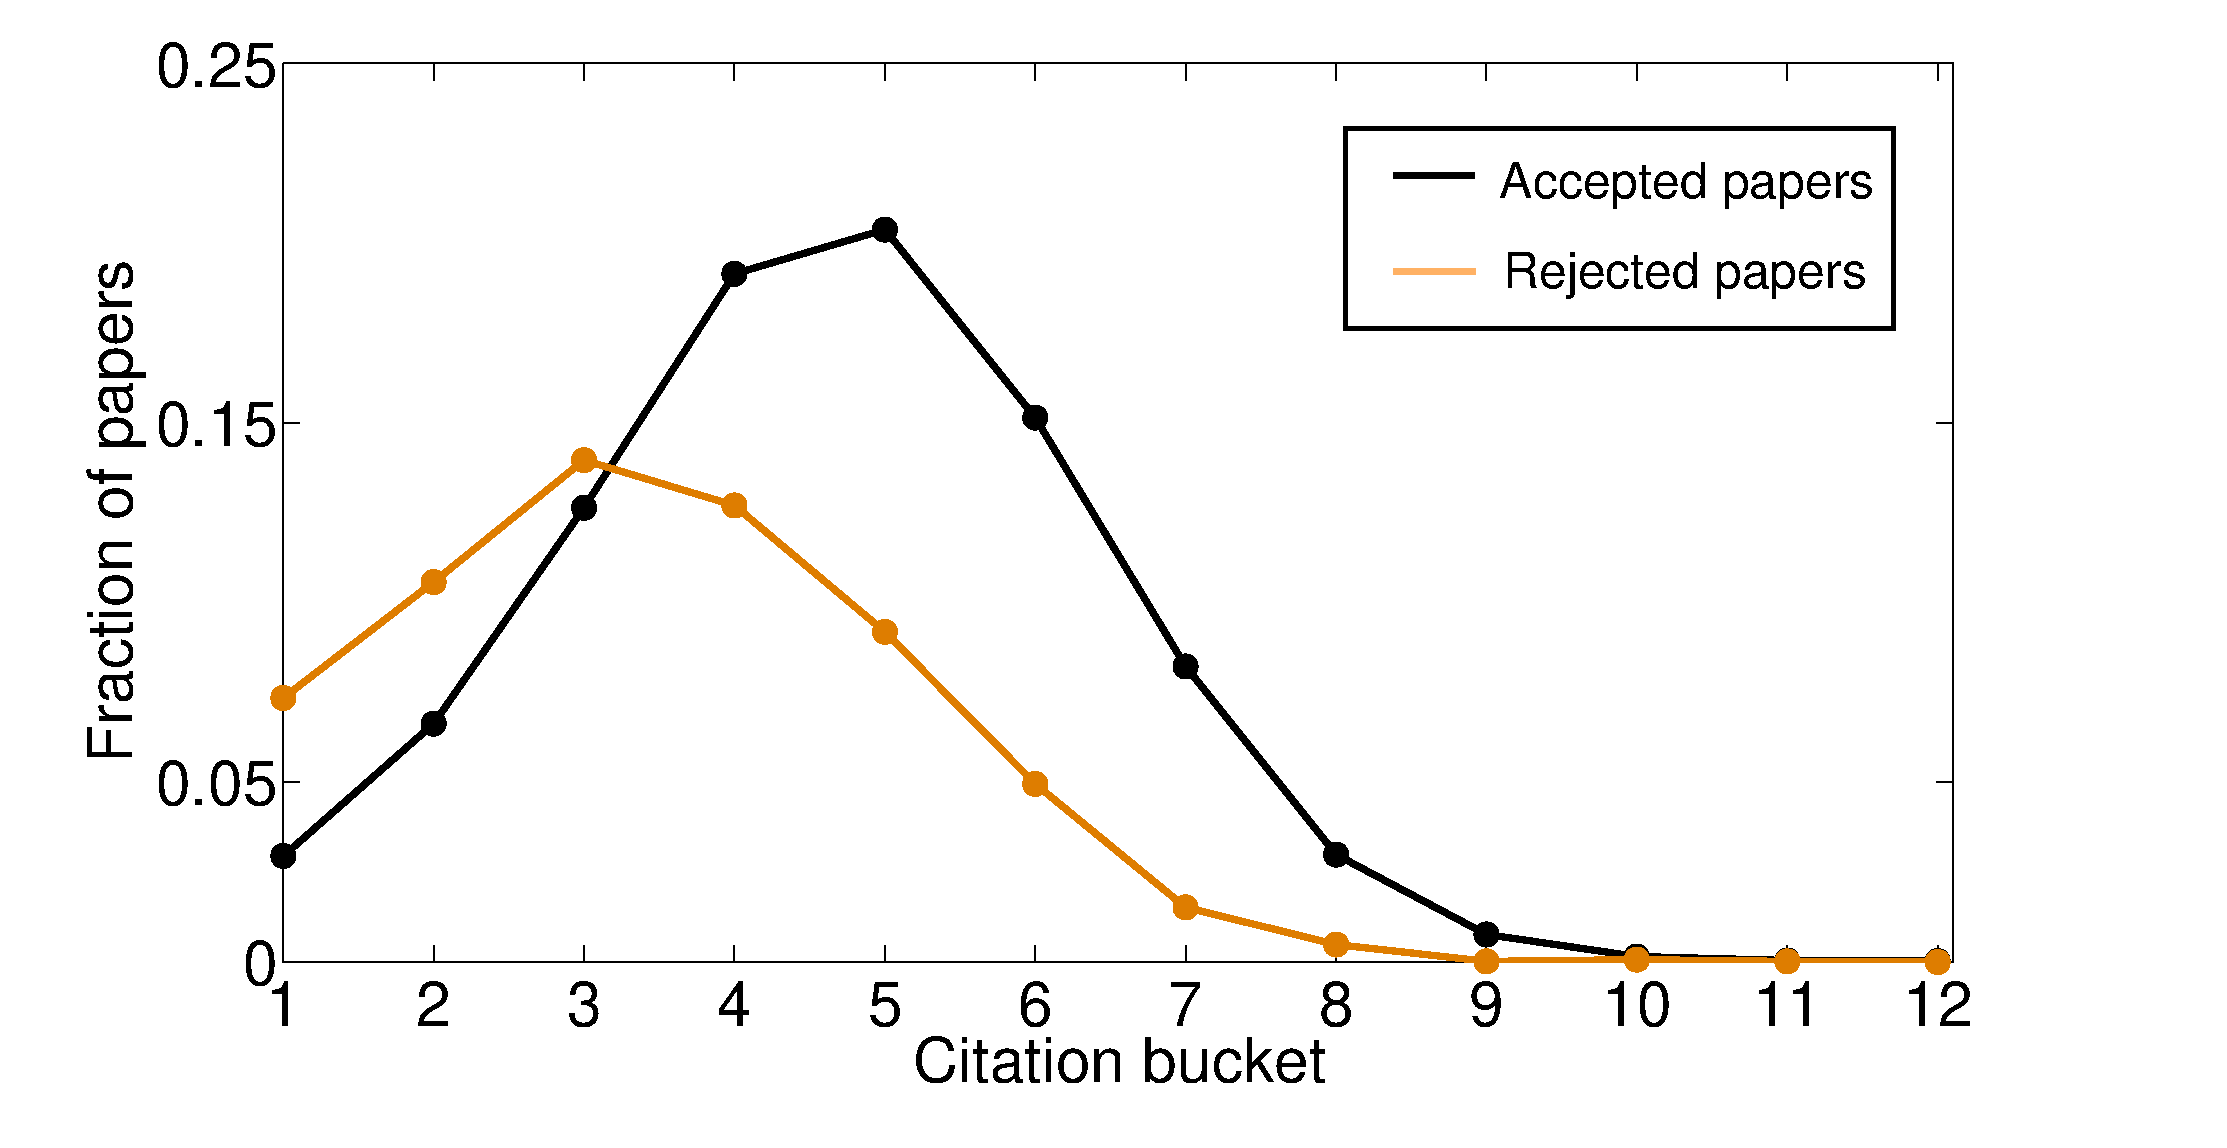
\includegraphics[scale=0.12]{./texfiles/Chapter_4/jcdl/figures/citation_bucket_frac_paper} & 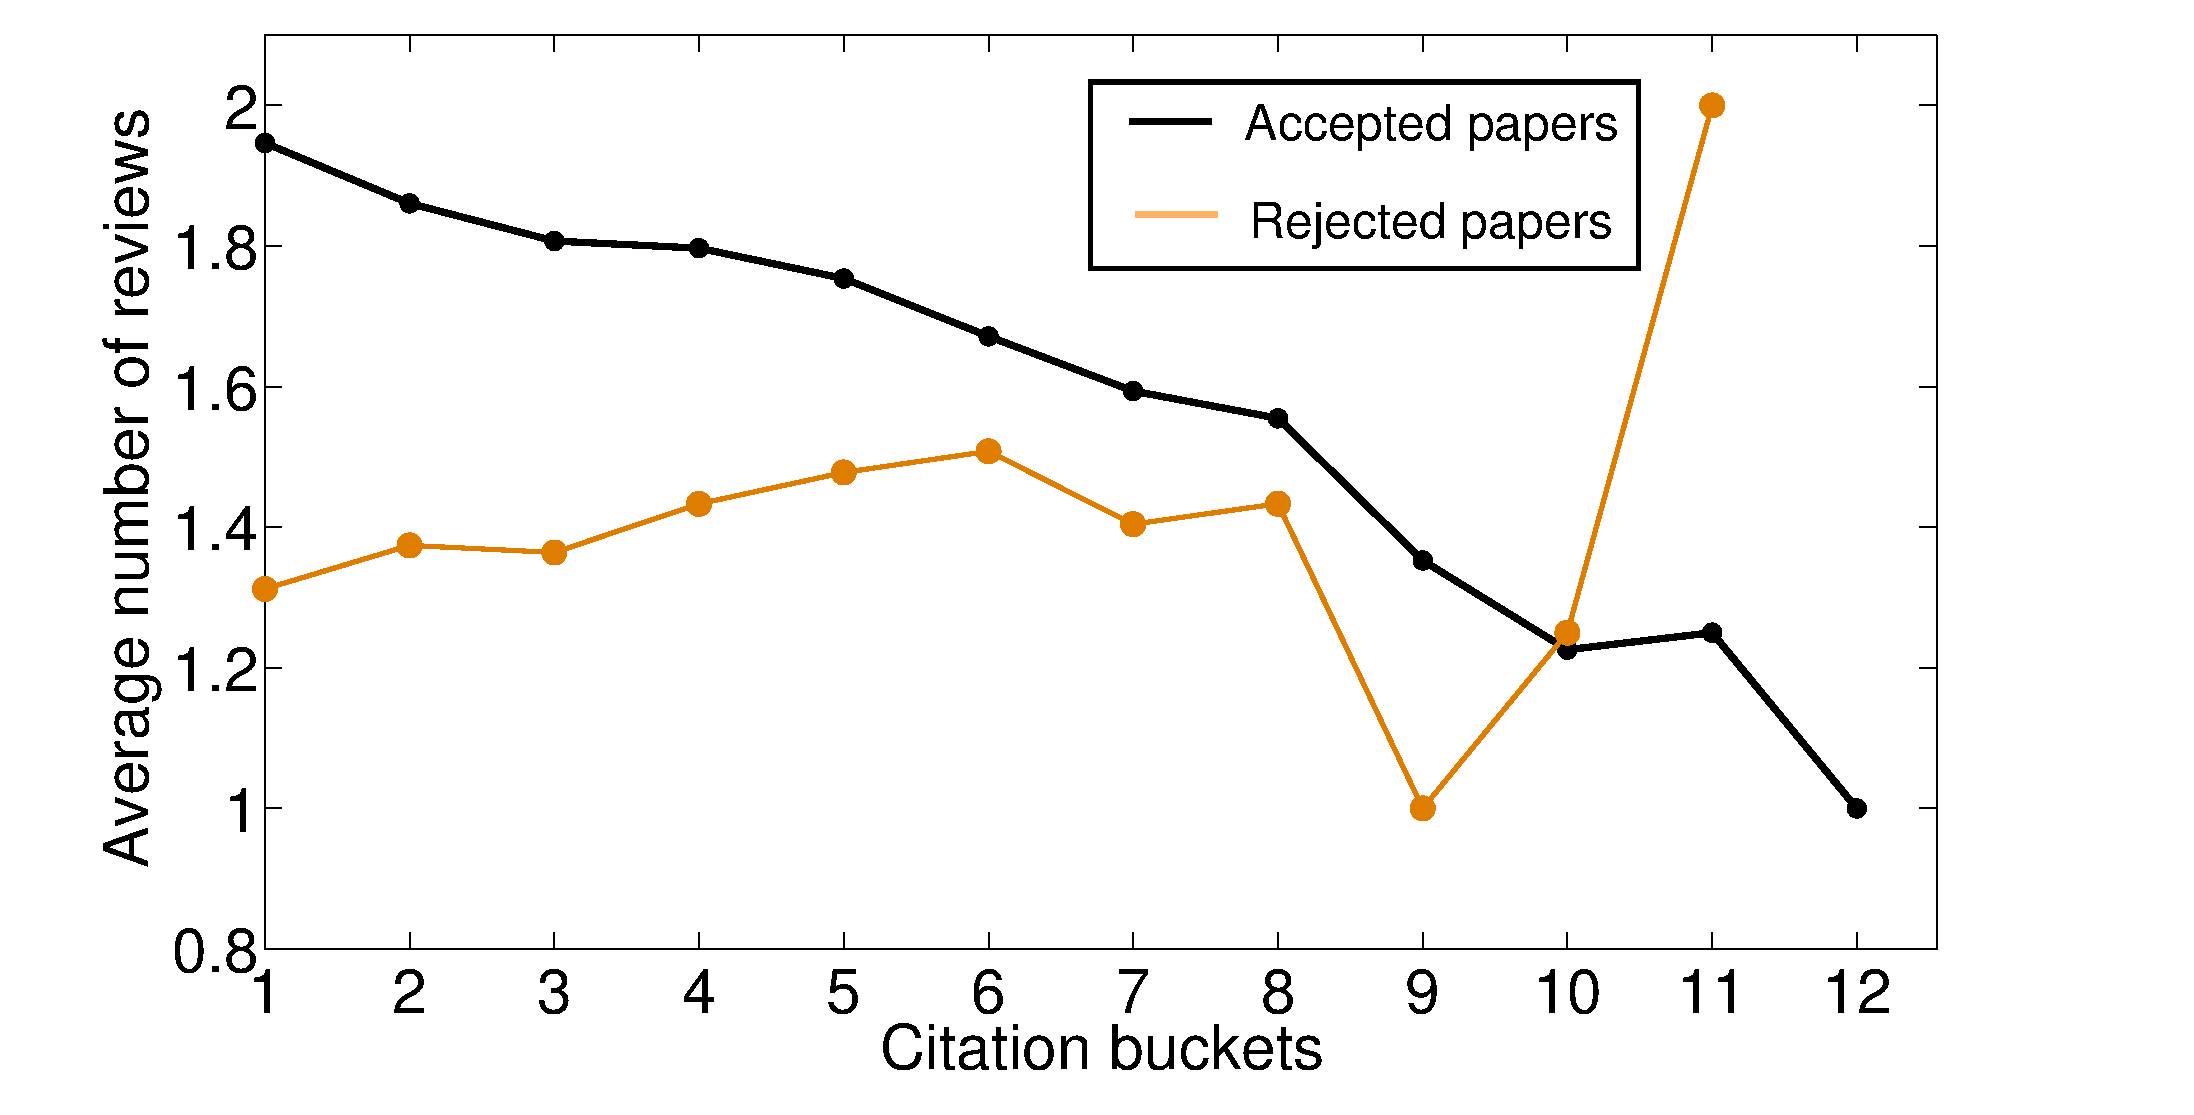
\includegraphics[scale=0.12]{./texfiles/Chapter_4/jcdl/figures/citation_bucket_reviews_all-eps-converted-to.pdf} & 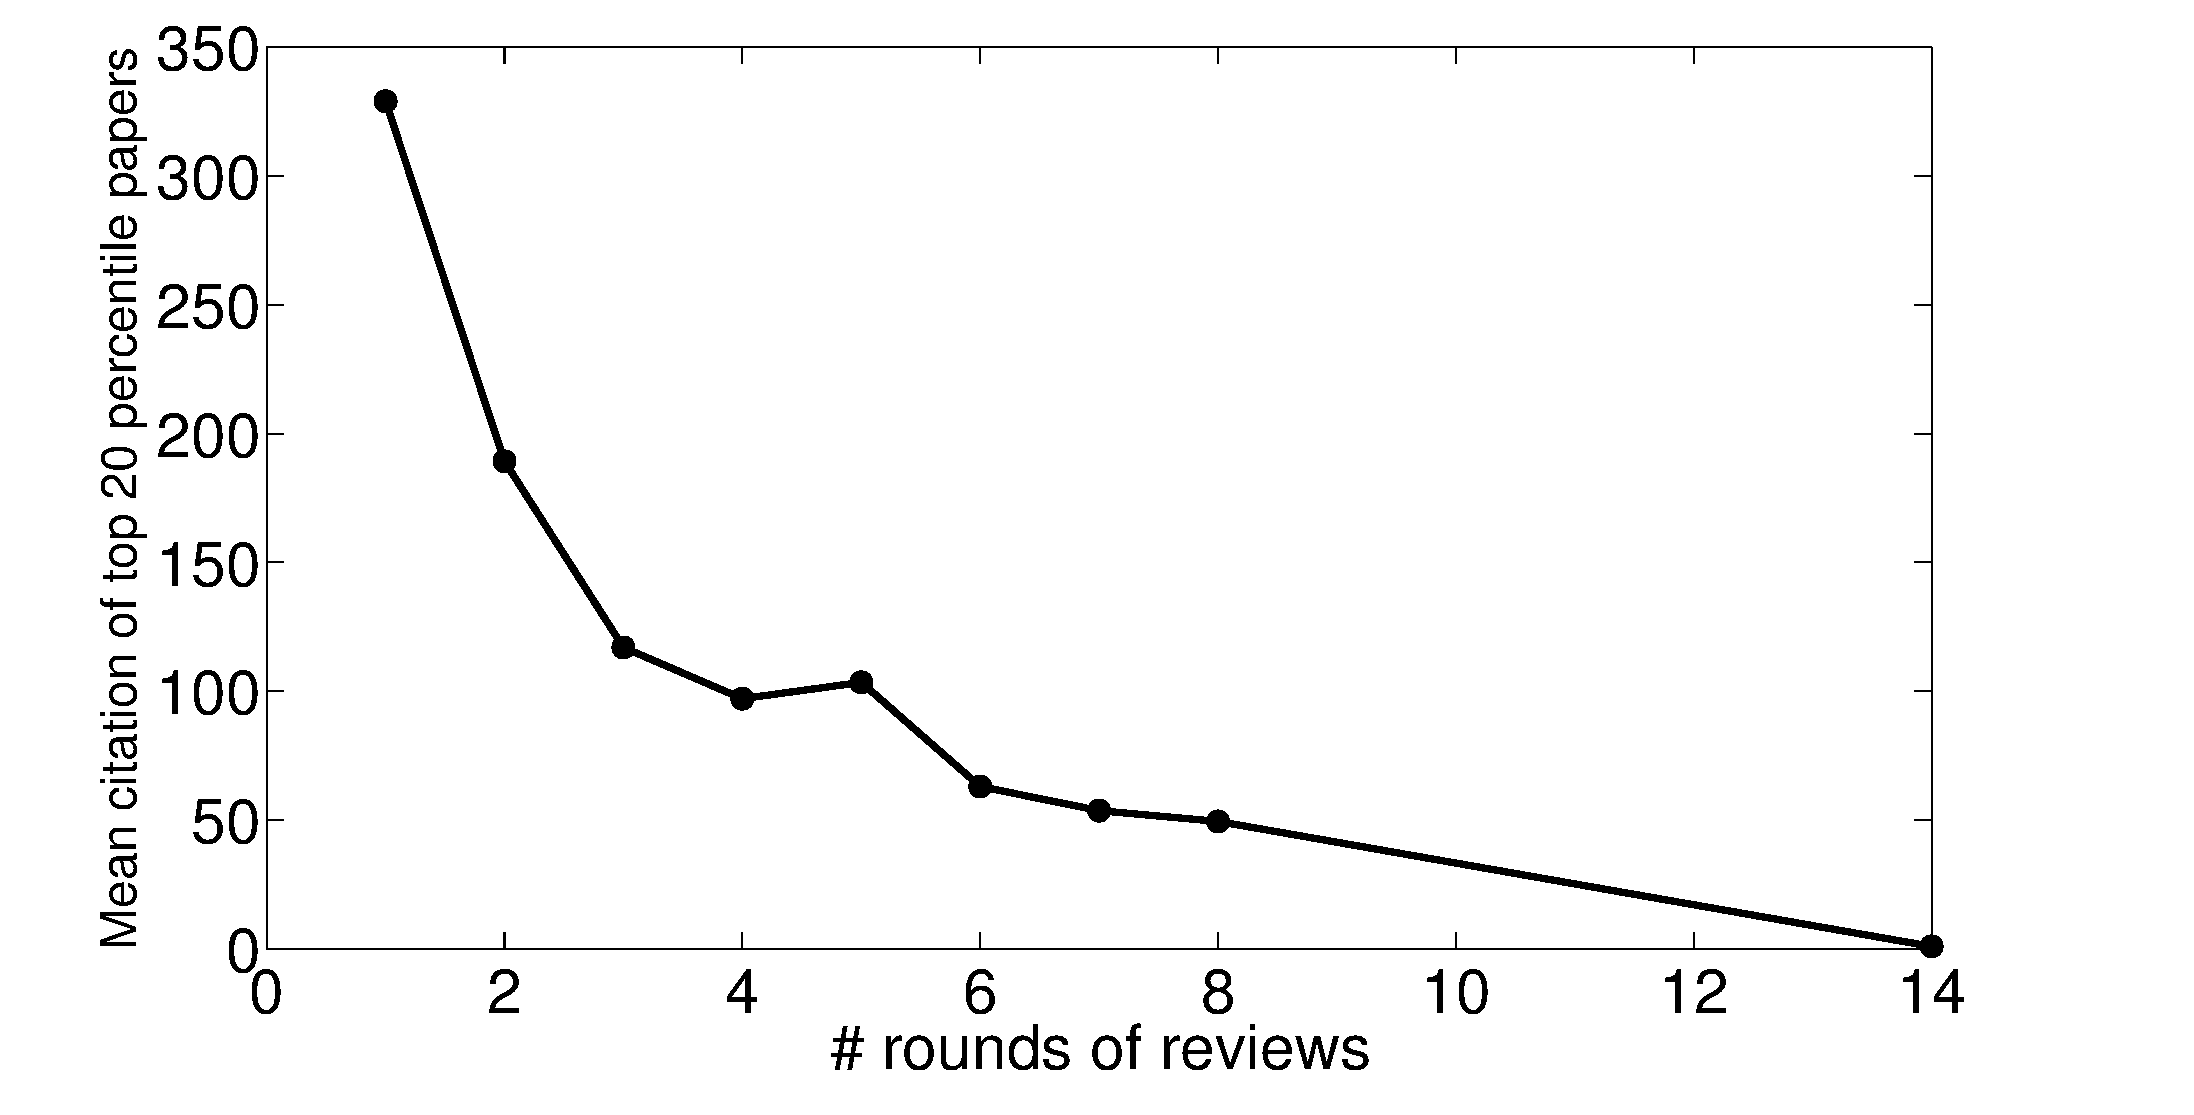
\includegraphics[scale=0.12]{./texfiles/Chapter_4/jcdl/figures/cit_rnd_rev-eps-converted-to.pdf}
 \end{tabular}
  \caption{{\bf (Left)} Fraction of accepted and rejected papers in different citation buckets. {\bf (Middle)} Average number of reviews for accepted and rejected papers in different citation buckets. For both {\bf (Left)} and {\bf(Middle) } bucket sizes are in increasing powers of 2. E.g. $\leq 1$, $2$, ($>2$ and $\leq 4$) and so on. {\bf (Right)} Average citation of the top 20 percentile  papers for a given number of rounds of review request.}
   \label{fig4}
   \vspace{4mm}
 \end{figure*}


We next check whether the {\bf review rounds} improve the quality of the paper. To this aim we segregate the papers based on the number of citations into different buckets and for each bucket we calculate the average number of reviews the papers received in that bucket. The bucket sizes are again in increasing powers of 2. Typically, the buckets are $\leq 1$, $2$, $(>2$ and $\leq 4)$ and so on. We plot the results in figure~\ref{fig4} {\bf (Middle)}. We observe that for accepted papers, the low cited ones on average tend to get accepted after more rounds of reviews while the high cited ones undergo lesser rounds of reviews before getting accepted. It can hence be concluded that going through the review process multiple times does not necessarily improve the quality of the papers much that are eventually accepted. For the rejected papers we observe a contrasting trend indicating that the review process indeed helped in improving the quality of the paper in the long run possibly enhancing the chances of its acceptance at a different venue later. For the accepted papers we further classify them based on the number of reviews they received and calculate the average citations of the top 20 percentile papers (ranked by citations) in each class (refer to figure~\ref{fig4} {\bf (Right)}). We observe that the average citation drops as the number of reviews increases further suggesting that papers accepted after higher number of reviews often fail to create a high citation impact. This indicates that the number of rounds of review could be an indicator of the long-term citation of the paper. 

\begin{figure}
\centering
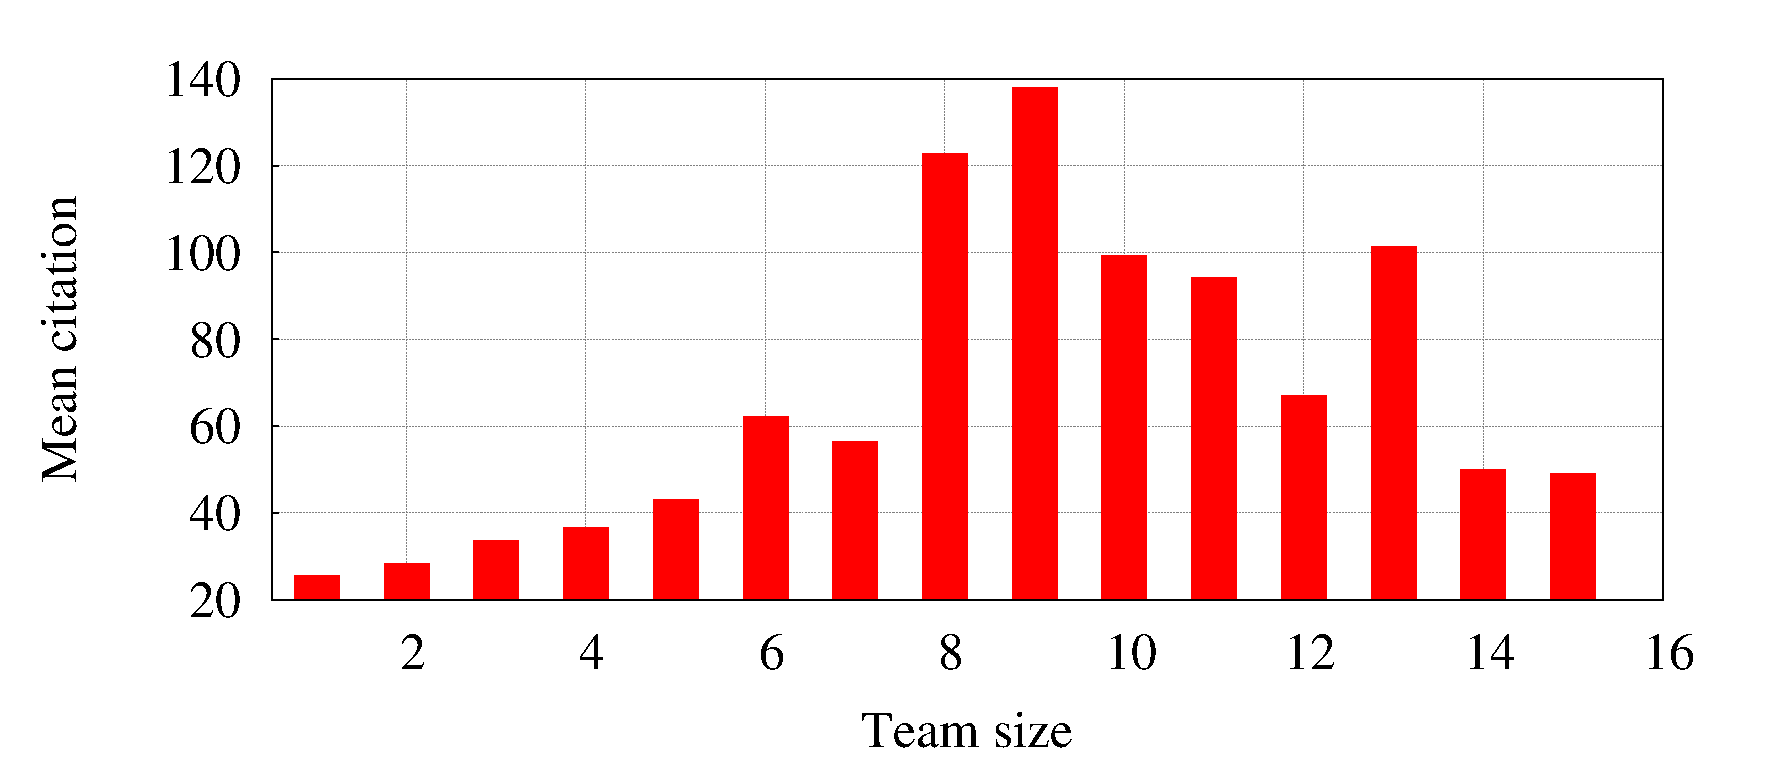
\includegraphics[scale  = 0.25]{./texfiles/Chapter_4/jcdl/figures/team_citation}
\caption{\label{team:citation} Average citation versus team size. Note that we segregate the papers based on the teams size and calculate the average citation.}
\vspace{4mm}
\end{figure}


\subsubsection*{Team size (TS)}
The authors in~\cite{chakraborty2014towards} hypothesized that there exits an optimal team size for which the citations received by the paper is maximum. We hence segregate the papers based on the team size and calculate the mean citation of the papers. We observe that team size 9 (refer to figure~\ref{team:citation}) is the optimal as the papers with 9 authors gets more citation on average.

\medskip


\begin{figure}
\centering
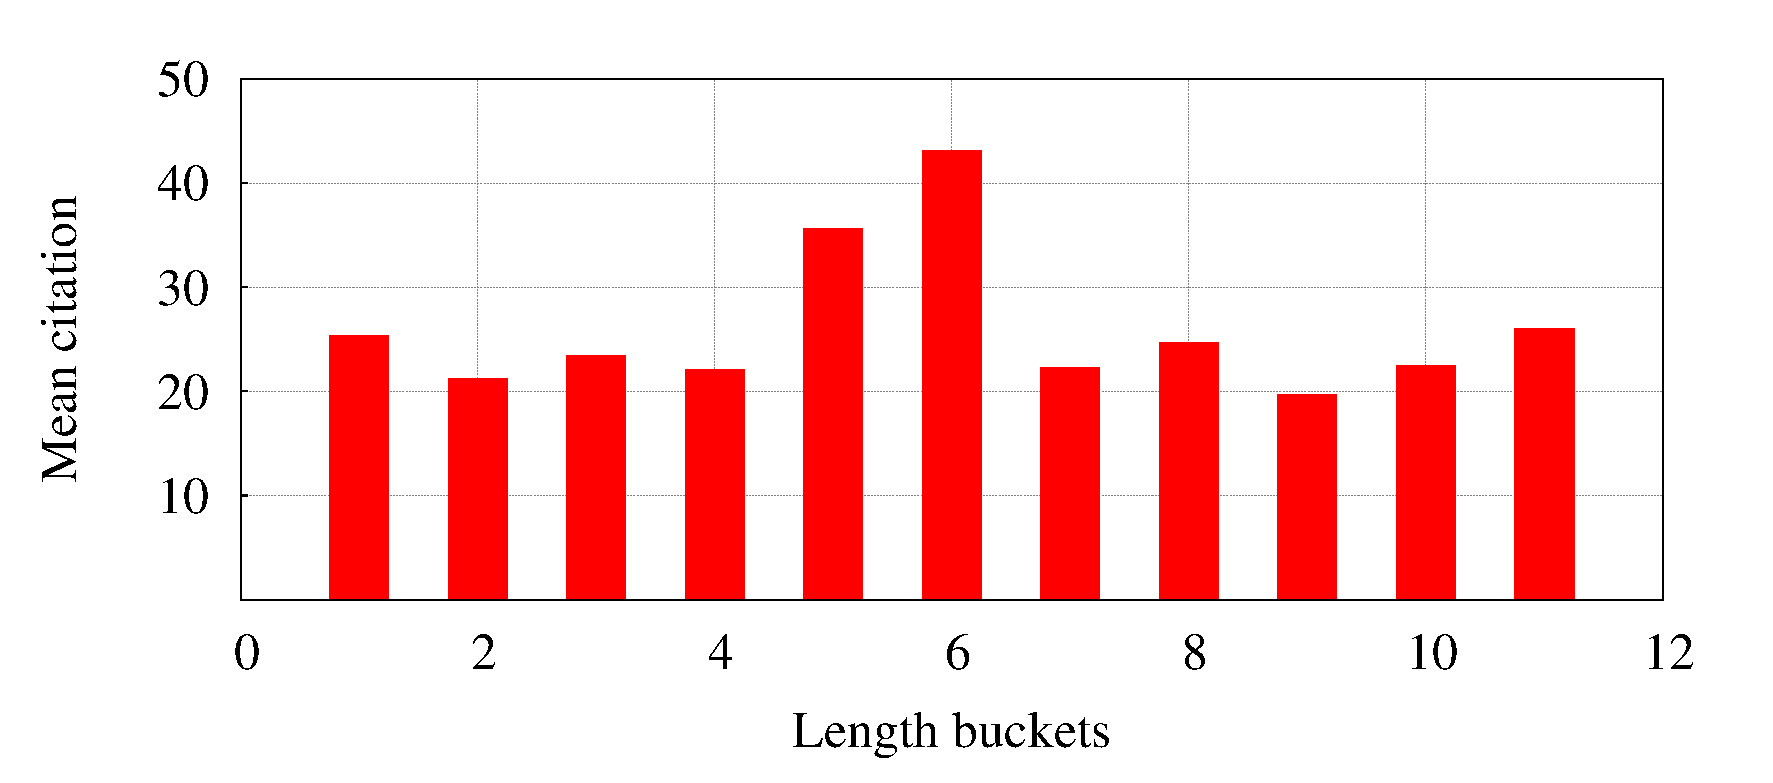
\includegraphics[scale=0.25]{./texfiles/Chapter_4/jcdl/figures/len_citation.eps}
\caption{Mean length of referee reports in terms of number of words at different rounds of review. Typically the buckets are $< 100$, ($\geq 100, < 200$) and so on}
\label{fig:length}
\vspace{3mm}
\end{figure}


\subsubsection{Review report based features}
\label{text_analysis}

In this subsection, we analyze whether certain features could be extracted from the reports sent by the reviewers that could be an indicator of the long-term citation of the paper. Note that we have two types of reports -- {\bf Referee report}: report sent by the assigned referee to the editors and {\bf Editor report}: report sent by the editor to the authors based on the referee report. We primarily focus on the referee reports as editorial reports are in almost all cases a reiteration of the referee reports.

\subsubsection*{Length of the reports (RL)}
We start by looking whether the length of the review reports sent by the reviewers are indicative of the quality and hence the long-term citation of the paper. To this aim we segregate the papers based on the length of the report and calculate the mean citation of each of these buckets. The lengths are bucketed with sizes typically $< 100$, ($\geq 100, < 200$) and so on. We observe that there exists an optimal length (between 500 and 600 words) for which the citation obtained by the corresponding paper is maximum  (refer to figure \ref{fig:length}). 


\subsubsection*{Sentiments (SNT)}
We next perform sentiment analysis on the review reports. To determine the sentiment of a report we use a method described in~\cite{montejo2012random} which performs a graph-based word sense disambiguation and lexical similarity analysis using a pre-existing knowledge base. A sentiment score of 0 indicates that the document is neutral, a positive score  indicates a positive sentiment and a negative score indicates a negative sentiment. 


\begin{figure}[htpb]
\centering
%\vspace{-5mm}
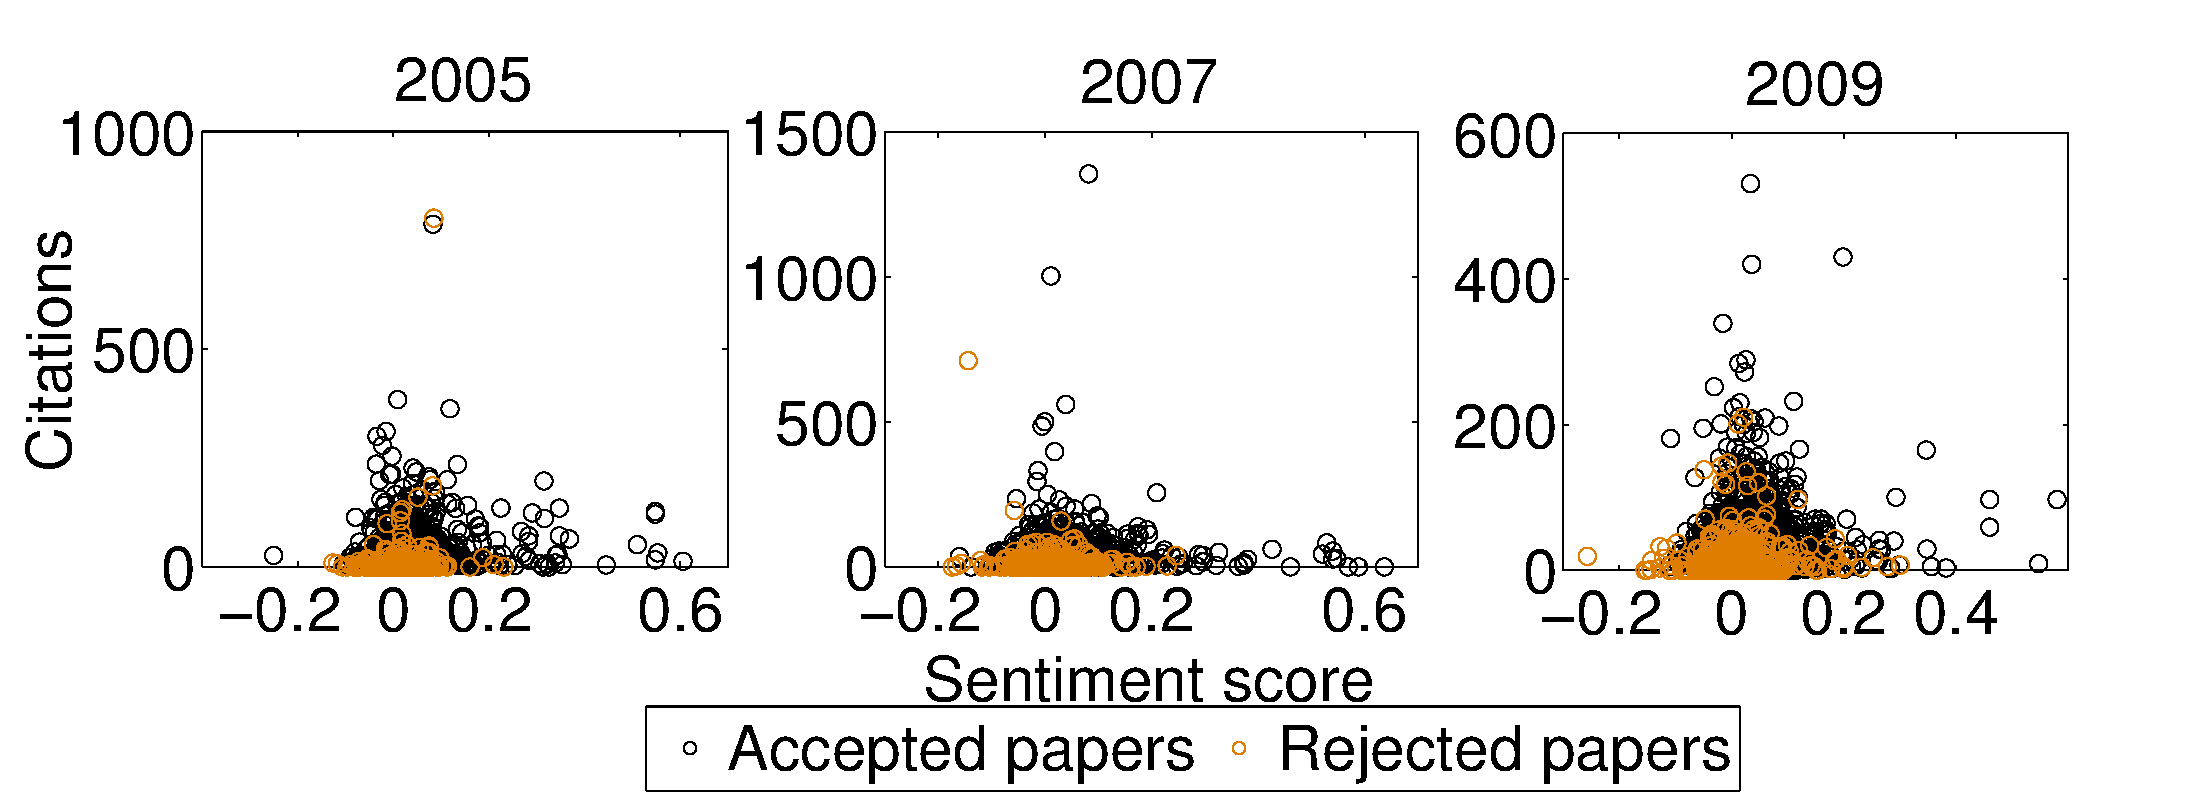
\includegraphics[scale=0.23]{./texfiles/Chapter_4/jcdl/figures/year_sent_cit-eps-converted-to.pdf}
\caption{Sentiment score versus citations for both accepted and rejected papers for the years 2005, 2007 and 2009. We find similar trends for other years as well.}
\label{fig12}
\vspace{3mm}
\end{figure}

To determine whether the overall sentiment of the reviews of a paper is related to the number of citations received by it, we plot for each paper (both accepted and rejected) the number of citations it received against the  sentiment score of the first round of review in figure~\ref{fig12}. Note that we segregate the papers based on the year of the publication or the rejection. We observe that the highly cited papers mostly have reviews with neutral or positive sentiment. Accepted papers with positive reviews are, on average, found to receive $25.27$ citations while those with negative reviews are found to receive $13.56$ citations.
However, there are cases where the accepted paper received highly positive reviews but was not cited. Conversely, there are cases where the sentiment was neutral but the paper garnered a large number of citations. Shown below are two such examples -- {\bf Case 1:} year of publication: 2006, sentiment score: 0.0234 (almost neutral), citations: 5812; {\bf Case 2:} year of publication: 2008, sentiment score: 0.65 (highly positive), citations: 6.


\begin{table}
\centering
\caption{Mean values of percentages of various categories of words in review reports of high and low cited papers where the means differ significantly.\vspace{3mm}}
\label{tab3}
\begin{tabular}{|l|l|l|l|}
\hline
Category                    & Dimension                                                   & \begin{tabular}[c]{@{}l@{}}High cited\\ papers\end{tabular} & \begin{tabular}[c]{@{}l@{}}Low cited\\ papers\end{tabular} \\ \hline \hline
\multirow{2}{*}{Linguistic} & Future tense                                                & 1.17                                                          & 1.05                                                         \\ \cline{2-4} 
                            & Negation                                                    & 0.72                                                          & 0.84                                                         \\ \hline
\multirow{4}{*}{Cognitive}  & Insight                                                     & 3.52                                                          & 3.16                                                         \\ \cline{2-4} 
                            & Causation                                                   & 2.60                                                          & 2.38                                                         \\ \cline{2-4} 
                            & Inclusive                                                   & 3.70                                                          & 3.43                                                         \\ \cline{2-4} 
                            & Exclusive                                                   & 1.28                                                          & 1.52                                                         \\ \hline
Affective                   & \begin{tabular}[c]{@{}l@{}}Positive \\ emotion\end{tabular} & 2.84                                                          & 2.70                                                         \\ \hline
\end{tabular}
\vspace{2mm}
\end{table}

For the rejected papers we observe that those which received neutral reviews but were rejected, tend to garner higher citations later compared to the ones which received negative reviews. There are certain exceptions as well, two of which are -- {\bf Case 1:} year of rejection: 2010, sentiment score: 0.27 (positive), citations: 1; {\bf Case 2:} year of rejection: 2007, sentiment score: -0.14 (negative), citations: 711.
Manual investigation of the review text shows that the papers which are highly cited after rejection were mainly rejected for not being in the scope of JHEP and not because of flawed results. 

\subsubsection*{Linguistic quality indicators (LQI)}

Here we check whether there are linguistic quality features present in the review reports which can serve as an indicator of the future impact of the paper. To our aim we use the LIWC\footnote{\url{http://liwc.wpengine.com/}} (Linguistic Inquiry and Word Count) text analysis tool~\cite{pennebaker2007development}. The tool provides, as output, percentage of words in different categories for an input text. The categories are broadly divided into linguistic (21 dimensions like pronouns, articles etc.), psychological (41 dimensions like affect, cognition etc.), personal concern (6 dimensions), informal language markers and punctuation apart from some general features like word count, words per sentence etc. We apply the LIWC tool on the review reports for our analysis and mainly focus on the linguistic and the psychological categories.
Next we check whether the LIWC features discussed earlier can also serve as indicators differentiating high and low cited papers. We rank the papers based on the number of citations they have received and consider the top 10\% as highly cited and the bottom 10\% as low cited papers. Note that we only consider the papers that were published before 2012 so that the papers have at least three years of citation history. In table~\ref{tab3} we report the mean percentage of words in different LIWC categories across all the papers (both high and low cited). We find several quality indicators here as well. The key observations are: (i) future tense is used more significantly in case of review reports of highly cited papers compared to low cited papers. On manually investigating the reviews of some of the highly cited papers we observe that statements like ``its result will become a useful addition to ..'' are prevalent; (ii) insightful and inclusive words are also used to a greater extent in review reports of highly cited papers compared to low cited papers; (iii) positive words are also more prevalent in highly cited papers as well.\\
Thus, these indicators show that the reviewers were, in many cases, indeed able to guess the quality of the paper as is evident from the review reports.






\noindent
\subsubsection{Reviewer based features}
\label{reviewer_analysis}

The success of the peer-review process is immensely dependent on the reviewers as they determine the quality of a paper and, consequently, the quality of the journal. We hence investigate certain reviewer behaviors (pointed out in~\cite{sikdar2016anomalies}) that could  be indicative of his/her performance.

\subsubsection*{Accept ratio (RAC)} For each reviewer we define a metric called accept ratio (this is different from the acceptance ratio defined in the previous section). Formally, the {\bf accept ratio} for reviewer $j$ is $accept\,ratio_{j}=\frac{accept_{j}}{accept_{j} + reject_{j}}$ 
where $accept_{j}$ and $reject_{j}$ respectively represent the number of papers reviewer $j$ accepted and rejected. The mean accept ratio across all the reviewers is $0.62$. An accept ratio of 1 for a reviewer would mean that he accepted all the papers that were assigned to him.

\begin{figure*}
\centering
\begin{tabular}{ccc}
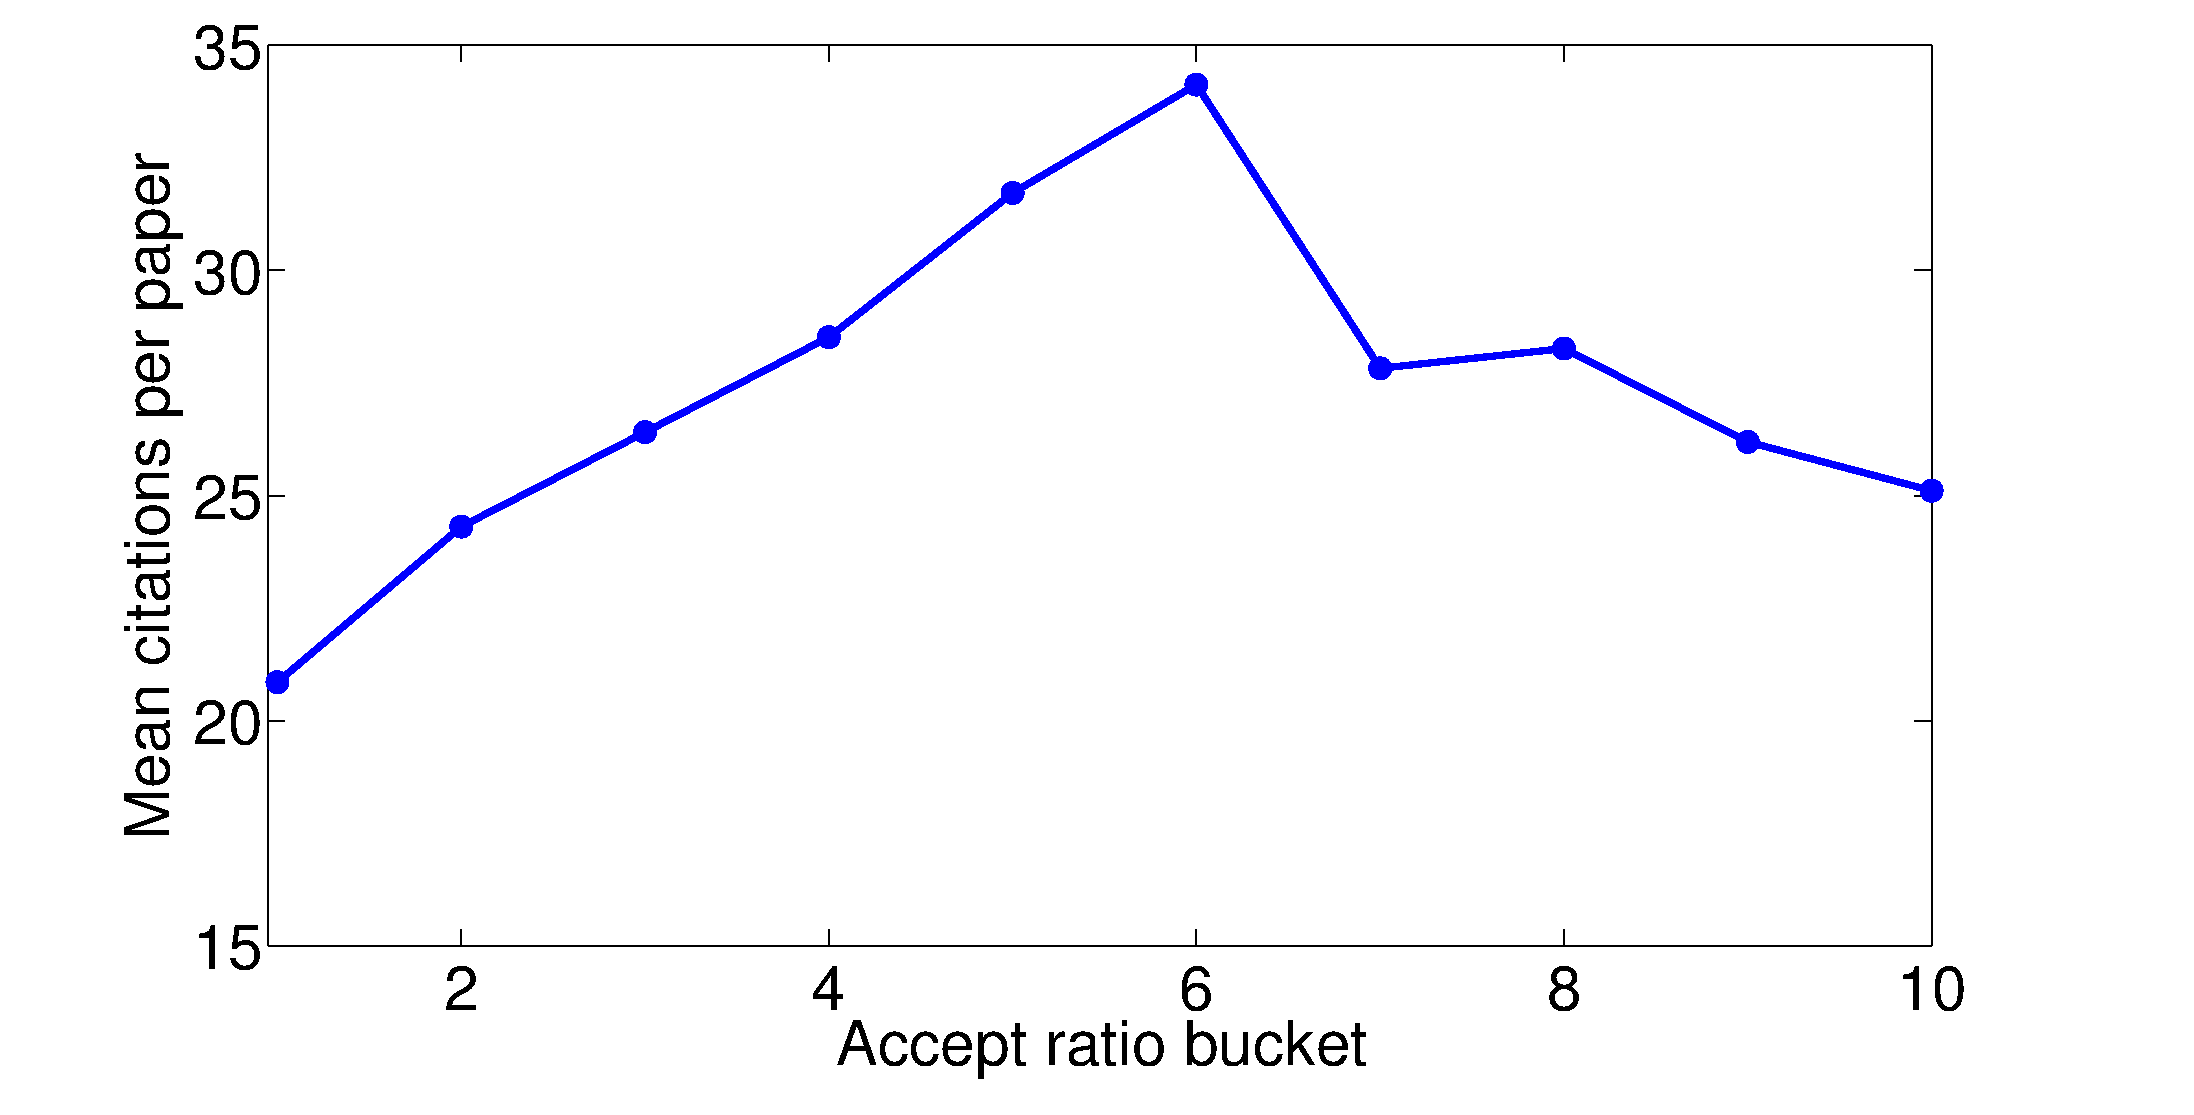
\includegraphics[scale=0.12]{./texfiles/Chapter_4/jcdl/figures/reviewer_citation_ratio-eps-converted-to.pdf} & 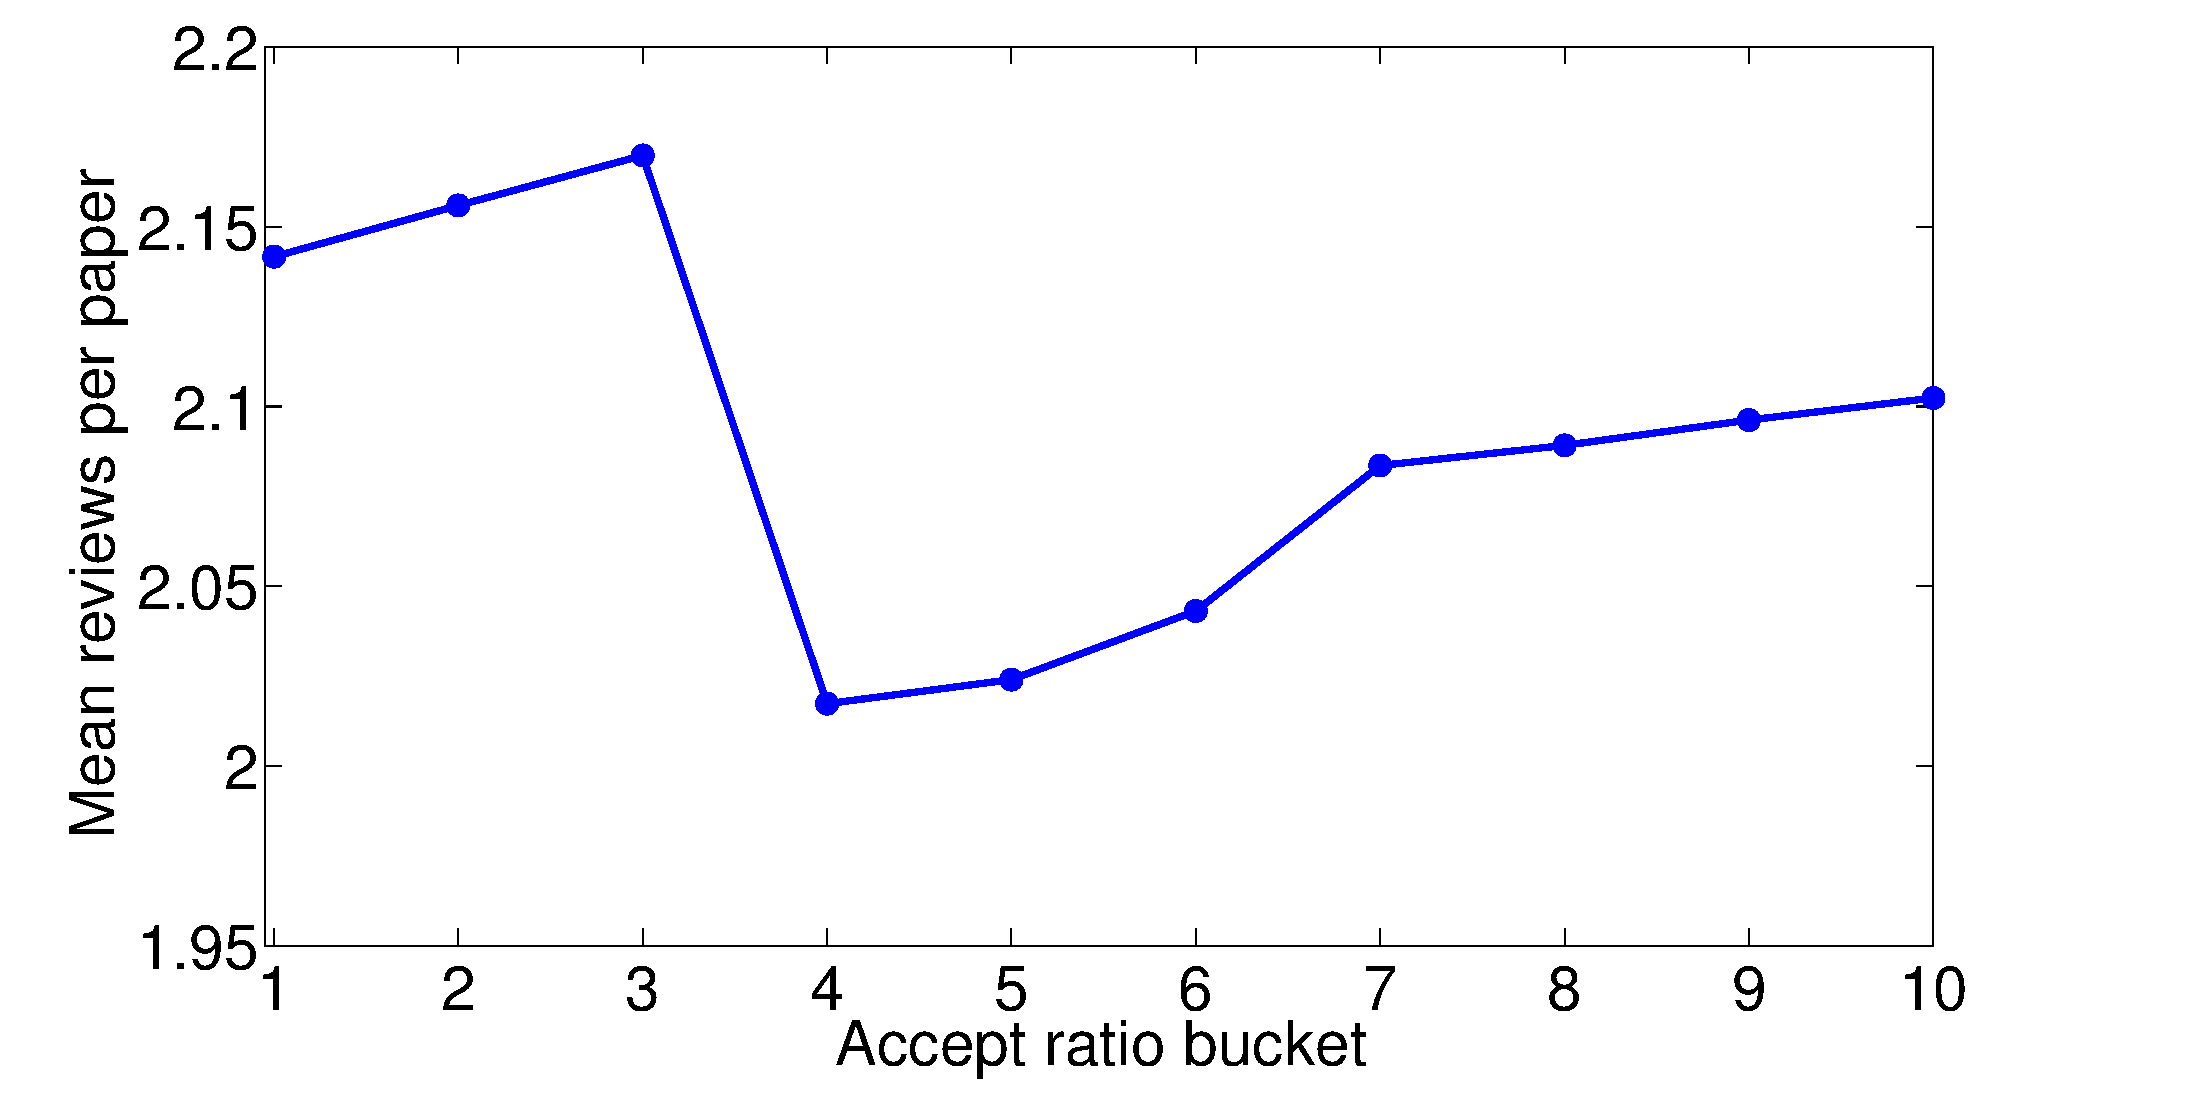
\includegraphics[scale=0.12]{./texfiles/Chapter_4/jcdl/figures/reviewer_review_ratio-eps-converted-to.pdf} & 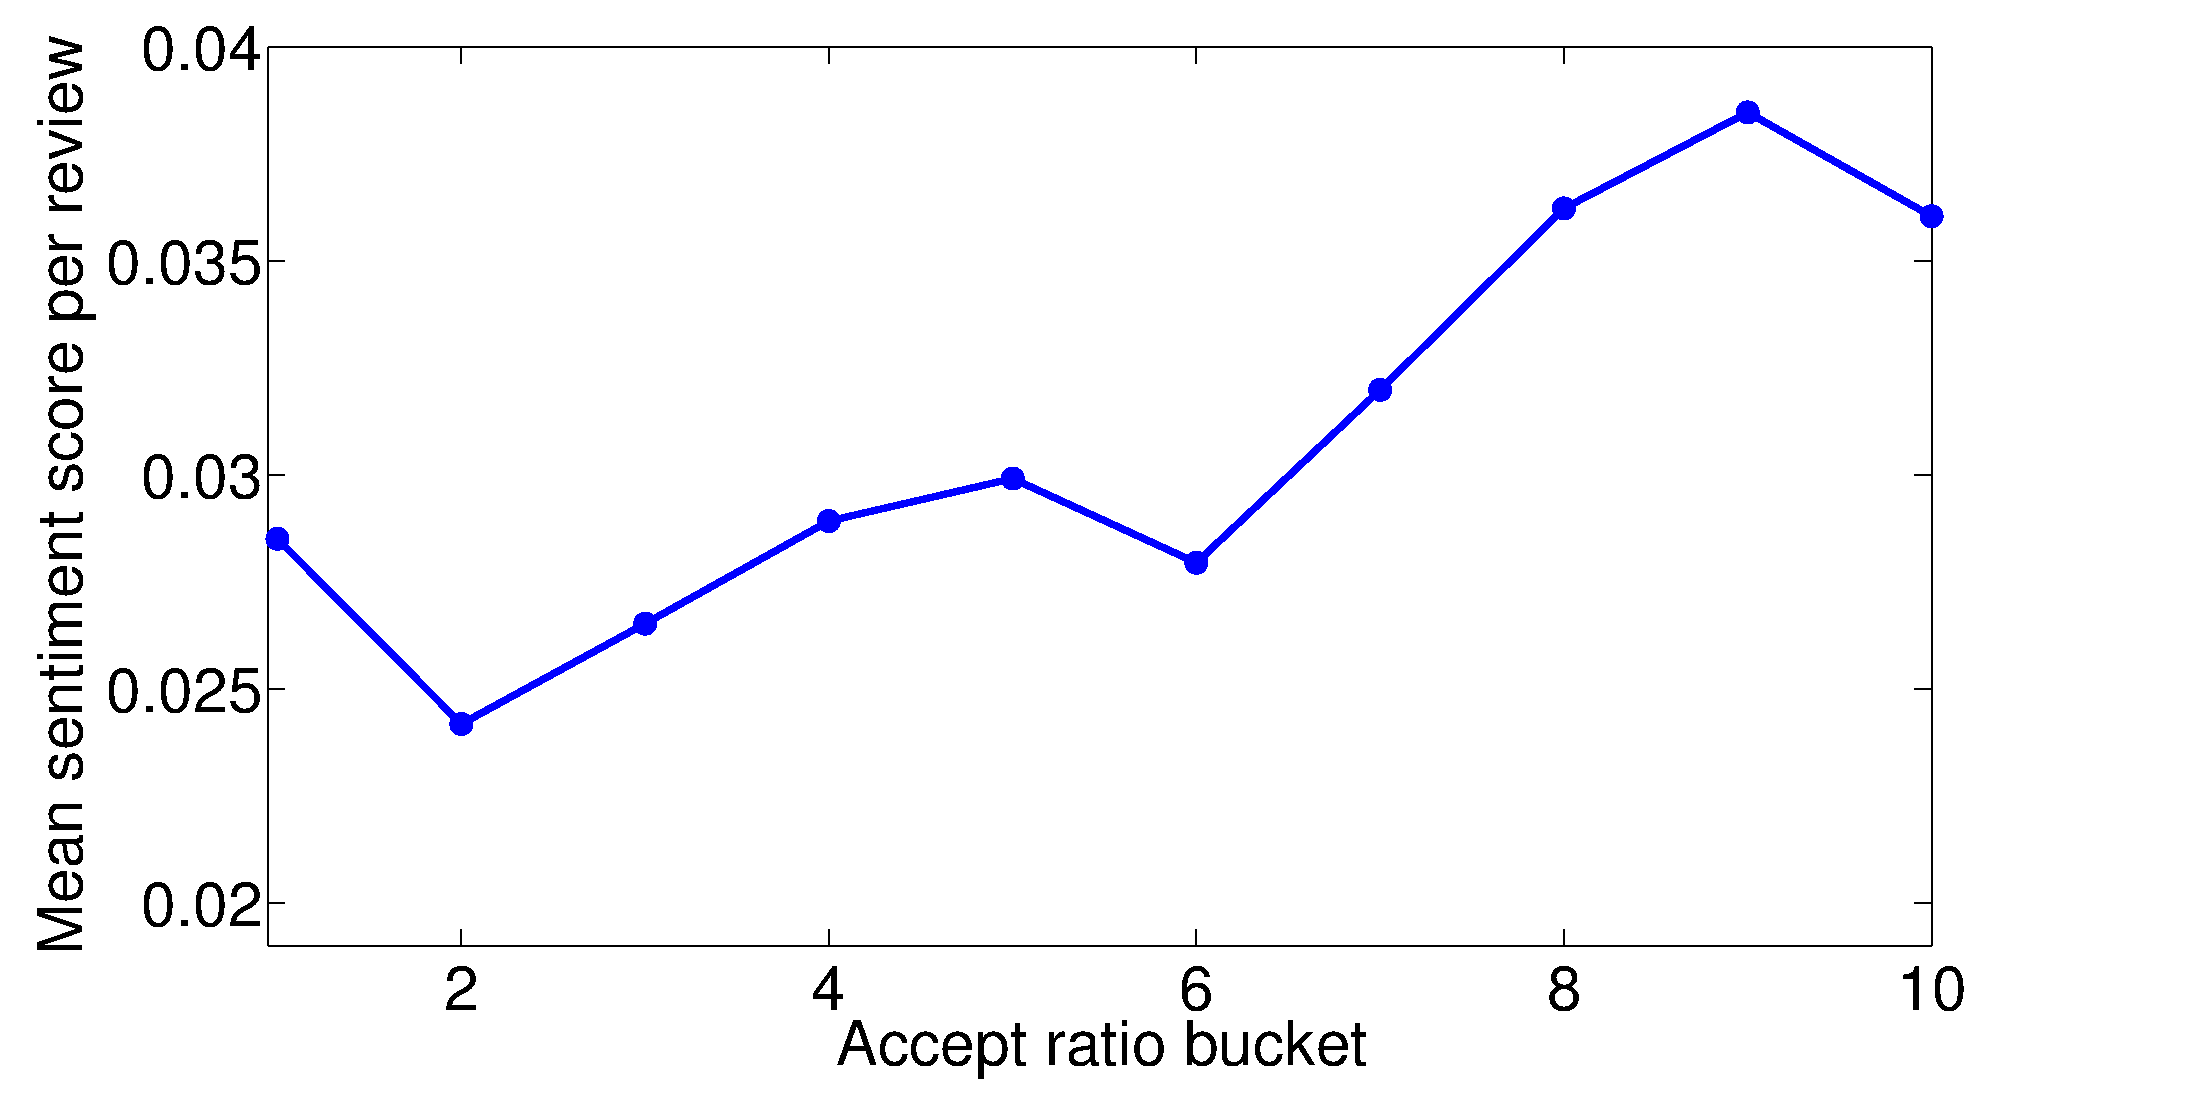
\includegraphics[scale=0.12]{./texfiles/Chapter_4/jcdl/figures/reviewer_sentiment_ratio-eps-converted-to.pdf}
\end{tabular}
\caption{{\bf (Left)} Mean number of citations per paper versus accept ratio. {\bf (Middle)} Mean number of reviews per paper versus accept ratio. {\bf (Right)} Mean sentiment score per paper versus accept ratio. Note that in each case we use accept ratio buckets where the buckets correspond to accept ratio ($\geq 0.1$ and $< 0.2$), ($\geq 0.2$ and $<0.3$) and so on.}
\label{fig16}
\vspace{3mm}
\end{figure*}


We start by investigating how well the reviewers were able to anticipate the quality of the paper. To this aim we segregate papers based on their assigned reviewer's accept ratio and calculate the mean number of citations received. In figure~\ref{fig16} {\bf (Left)} we plot the number of citations per paper given the accept ratio of the assigned reviewer. We observe that most cited papers were reviewed by reviewers with accept ratio between 0.6 and 0.7. Surprisingly, the papers reviewed by reviewers with very low and very high accept ratio tend to garner less citations. This indicates that some papers could have been accepted just because the assigned reviewer is oriented to accept most of the papers. In fact, manual inspection indicates that many of the rejected papers that garnered large number of citations later on were mostly reviewed by reviewers with low accept ratio. We further investigate the number of reviews a reviewer with a given accept ratio suggests before he accepts or rejects a paper. For this we again segregate the papers based on the assigned reviewers accept ratio and calculate the number of rounds of reviews, these papers received on average. We present the results in figure~\ref{fig16} {\bf (Middle)}. Since in most of the cases the same reviewer is assigned in each round of review, we observe that reviewers with a low accept ratio tend to recommend more rounds of reviews while those with higher accept ratio tend to suggest lesser number of review rounds. This indicates that the reviewers with low accept ratio often fail to improve the quality of the paper as is evident from the mean number of citations these papers receive albeit dragging the paper through multiple rounds of reviews.


To complete the analysis we also investigate the average sentiment score of the papers based on the accept ratio of the assigned reviewers. In figure~\ref{fig16} {\bf (Right)} we plot the average sentiment score of the papers with similar accept ratio of the assigned reviewer. We observe an increasing trend indicating that the reviewers with very high accept ratio always tend to give more positive reviews as compared to others with lower accept ratio. \iffalse Note that we also repeat the analysis for the small set of editors separately; in all cases the results show exactly similar trends as in case of reviewers.\fi 


\begin{figure}
\centering
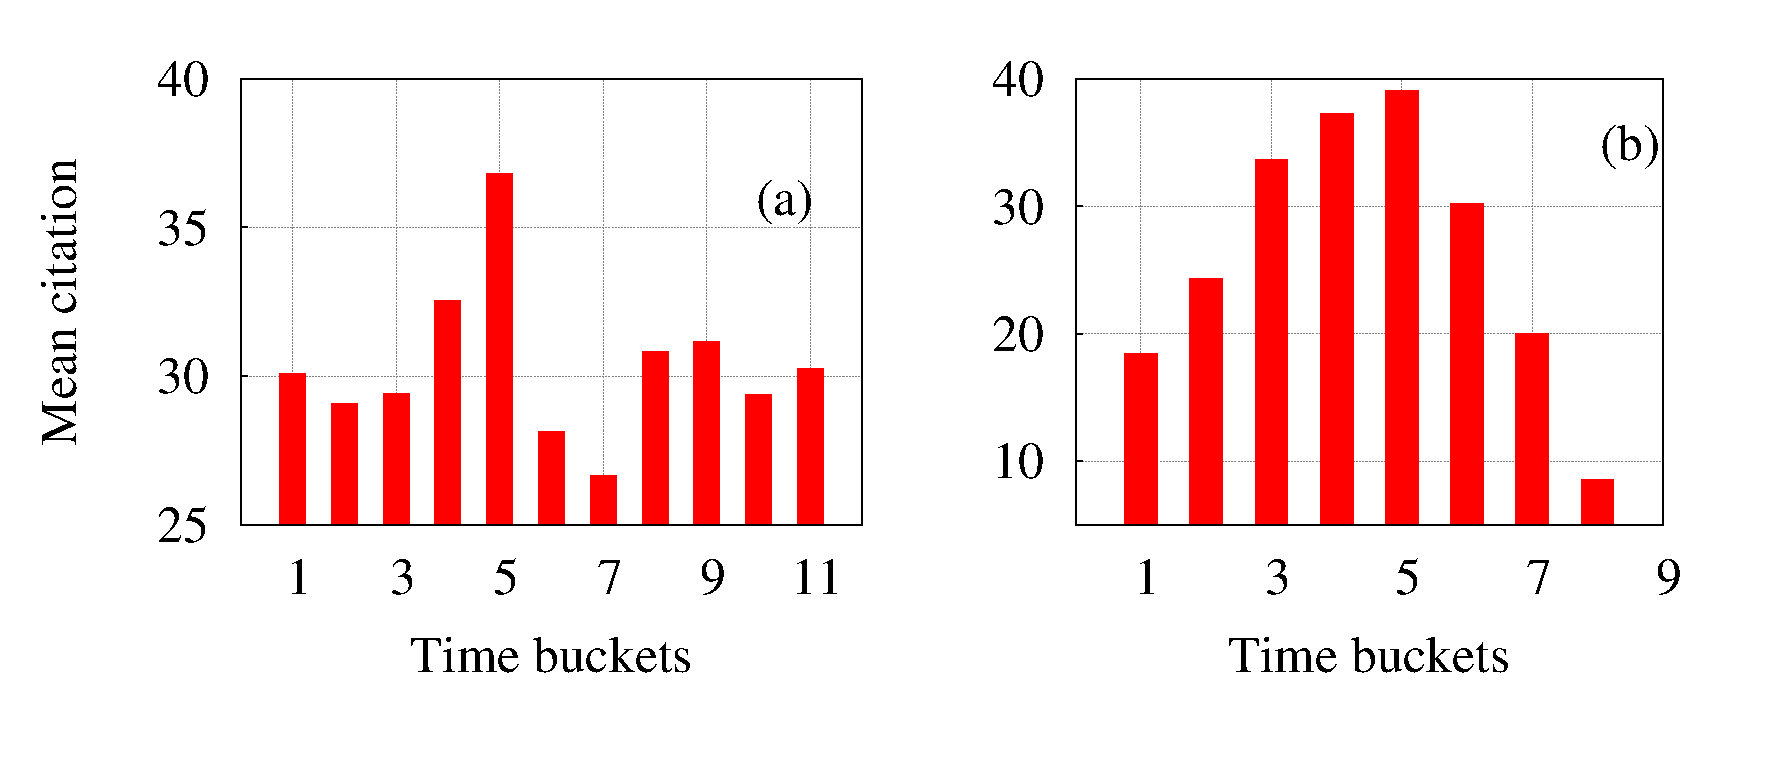
\includegraphics[scale = 0.28]{./texfiles/Chapter_4/jcdl/figures/rev_all.eps}
\caption{\label{fig:rev} Mean citation of the papers versus (a) time since the last assignment for the assigned reviewer and (b) time taken by the reviewer to send the report. Note that for both the cases the times are divided into equi-sized buckets. For (a) bucket sizes are 100 each while for (b) it is 25.}
\end{figure}

\subsubsection*{Time since last assignment (TA)}

In lines of~\cite{sikdar2016anomalies} we consider the time (in number of days) since the last assignment for the assigned reviewer as an indicator of reviewer's performance and hence an indicator of the long-term citation of the paper. To verify our hypothesis we segregate the papers based on the assigned reviewer's time till last assignment and calculate the mean citation. The times are bucketed with bucket size typically $< 100$, ($\geq 100, < 200$) and so on. We observe in figure~\ref{fig:rev} (a) that there does exist an optimal time for which the citation of the accepted paper is maximum. Further if the time since last assignment is too low or too high the long-term citation is low.   

\subsubsection*{Delay in submitting the report (DR)}

We further check whether the time taken by the assigned reviewer in submitting the report is also as an indicator for his performance and hence that of the long-term citation of the paper. To this aim we calculate for each paper the time between assigned reviewer acknowledging to review the paper and the reviewer sending back the report. The papers are segregated based on this time and then the mean citation is calculated. 
We binned the times using typical bucket sizes being $>25$, $(\geq 25, < 50)$ and so on. We observe from figure~\ref{fig:rev} (b) that the citation is maximum when the reviewer sent back the report between 50 and 75 days. The citations are comparatively less if the time is too high as well as too low. 

\medskip




%\vspace{-8mm}
\subsection{Prediction results}
\label{performance_measure}

\begin{table*}[]
\centering
\caption{The F-statistics value for all the features used for predicting the long-term citation of the paper.}
\label{tab:f_score}
 \begin{adjustbox}{max width=\textwidth}
\begin{tabular}{|l|l|l|l|l|l|l|l|l|l|l|l|l|l|l|}
\hline
Feature      & Deg  & BC    & CC    & Clus  & PR    & RR   & TS   & RL   & SNT  & AR    & AP    & RAC  & TA   & DR   \\ \hline
F-statistics & {\bf 26.1} & {\bf 29.21} & {\bf 27.72} & {\bf 17.82} & {\bf 23.34} & 6.17 & {\bf 25.6} & 14.1 & 0.94 & {\bf 18.52} & {\bf 16.49} & 3.49 & 8.68 & 7.59 \\ \hline
\end{tabular}
\end{adjustbox}
\vspace{4mm}
\end{table*}

\begin{table*}[]
\centering
\caption{The F-statistics value for all author related features for predicting the long-term citation of the paper.}
\label{tab:fscore_author}
\begin{tabular}{|l|l|l|l|l|l|l|l|l|}
\hline
Features     & AS   & AC    & AF    & Age   & AAR   & ACD   & ACA   & ATD   \\ \hline
F-statistics & 26.3 & 19.23 & 18.67 & 25.42 & 22.15 & 25.78 & 23.32 & 17.68 \\ \hline
\end{tabular}
\vspace{4mm}
\end{table*}

In this section we design a regression model to calculate the long-term citation impact of a paper. 
We perform our prediction for papers that were accepted in JHEP between 2007 and 2012. Note that for each paper, its citation till 2015 is available. Hence papers published in 2004 would have a higher citation on average compared to papers which were published in 2010 (say) due to higher exposure time. Thus, instead of calculating  the exact citation value we predict the citation rank (for each year we rank the papers based on the citations they have accrued till 2015). Further note that the papers are sorted based on the date of submission and given a paper we construct the reviewer-reviewer interaction network until its submission date (excluding). This ensures that there is no data leakage. Similarly for supporting features like acceptance ratio of an author we consider information only up to his/her last submission. 

\noindent{\bf Network features only:} Considering only the network features, we obtain the best result using support vector regression (RBF kernel) with parameters $C=100$ and $\gamma=0.01$. We perform a 10-fold cross-validation and obtain a high $R^2$ of {\bf 0.79} and a low $RMSE$ of {\bf 0.496}. 

\noindent{\bf Network + supporting features:} Considering both the network and the supporting features we obtain a further overall improvement. In specific, using support vector regression (RBF kernel) we obtain a high $R^2$ of {\bf 0.81} and a low $RMSE$ of {\bf 0.46}. In this case we set the parameters $C=100$ and $\gamma=0.02$. We further calculate the $F$-Statistic values for all the features used in the regression task (refer to tables~\ref{tab:f_score} and \ref{tab:fscore_author}) and observe that the network features, are in general, are more suited to the task of prediction.


Thus our system is correctly able to predict the citation rank of the paper. We believe our system could be useful in assisting the editors in deciding whether to accept or reject the papers especially in cases where the reports are contradictory. 
\medskip



\noindent
%\vspace{-3mm}
\section{Irregular cases}

\begin{figure}
\centering
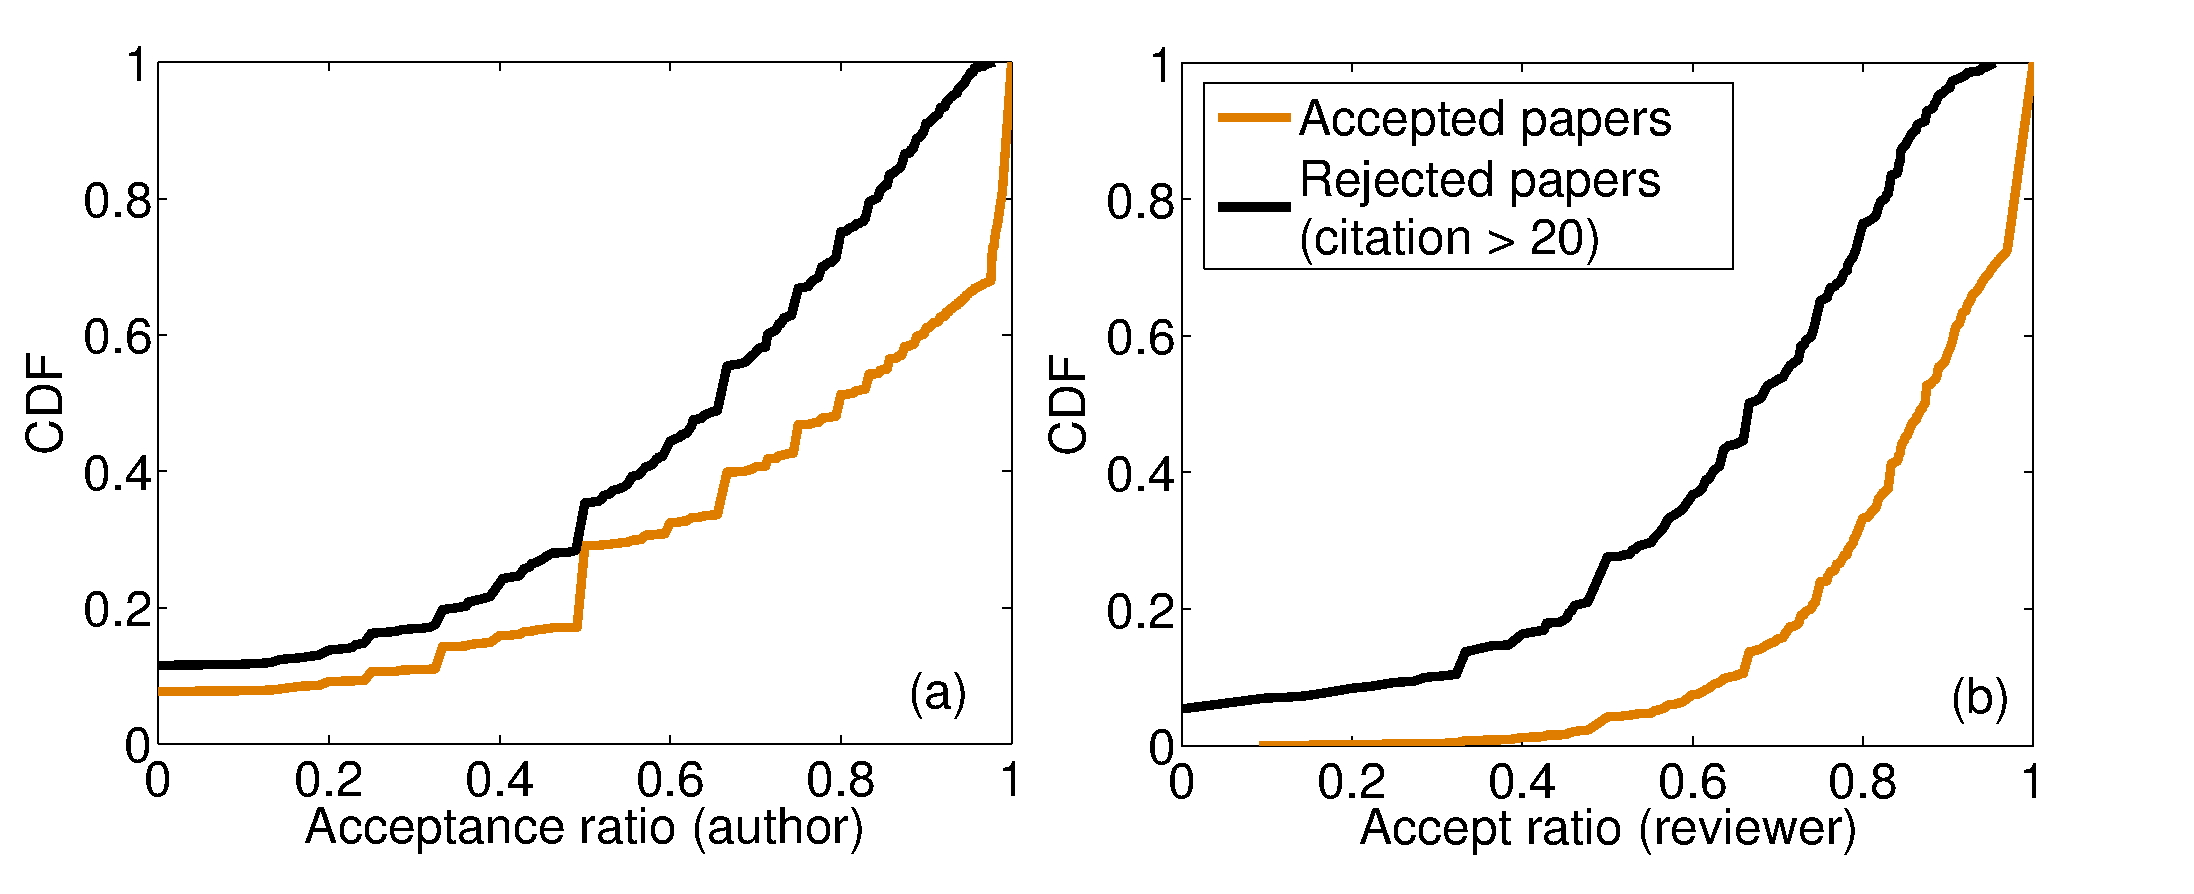
\includegraphics[scale=0.17]{./texfiles/Chapter_4/jcdl/figures/highly_cited_rejected-eps-converted-to.pdf}
\caption{CDF of (a) acceptance ratio of authors and (b) accept ratio of reviewers for accepted papers and highly cited rejected papers.}
\label{fig10}
%\vspace{-1mm}
\end{figure}

\begin{figure}
\centering
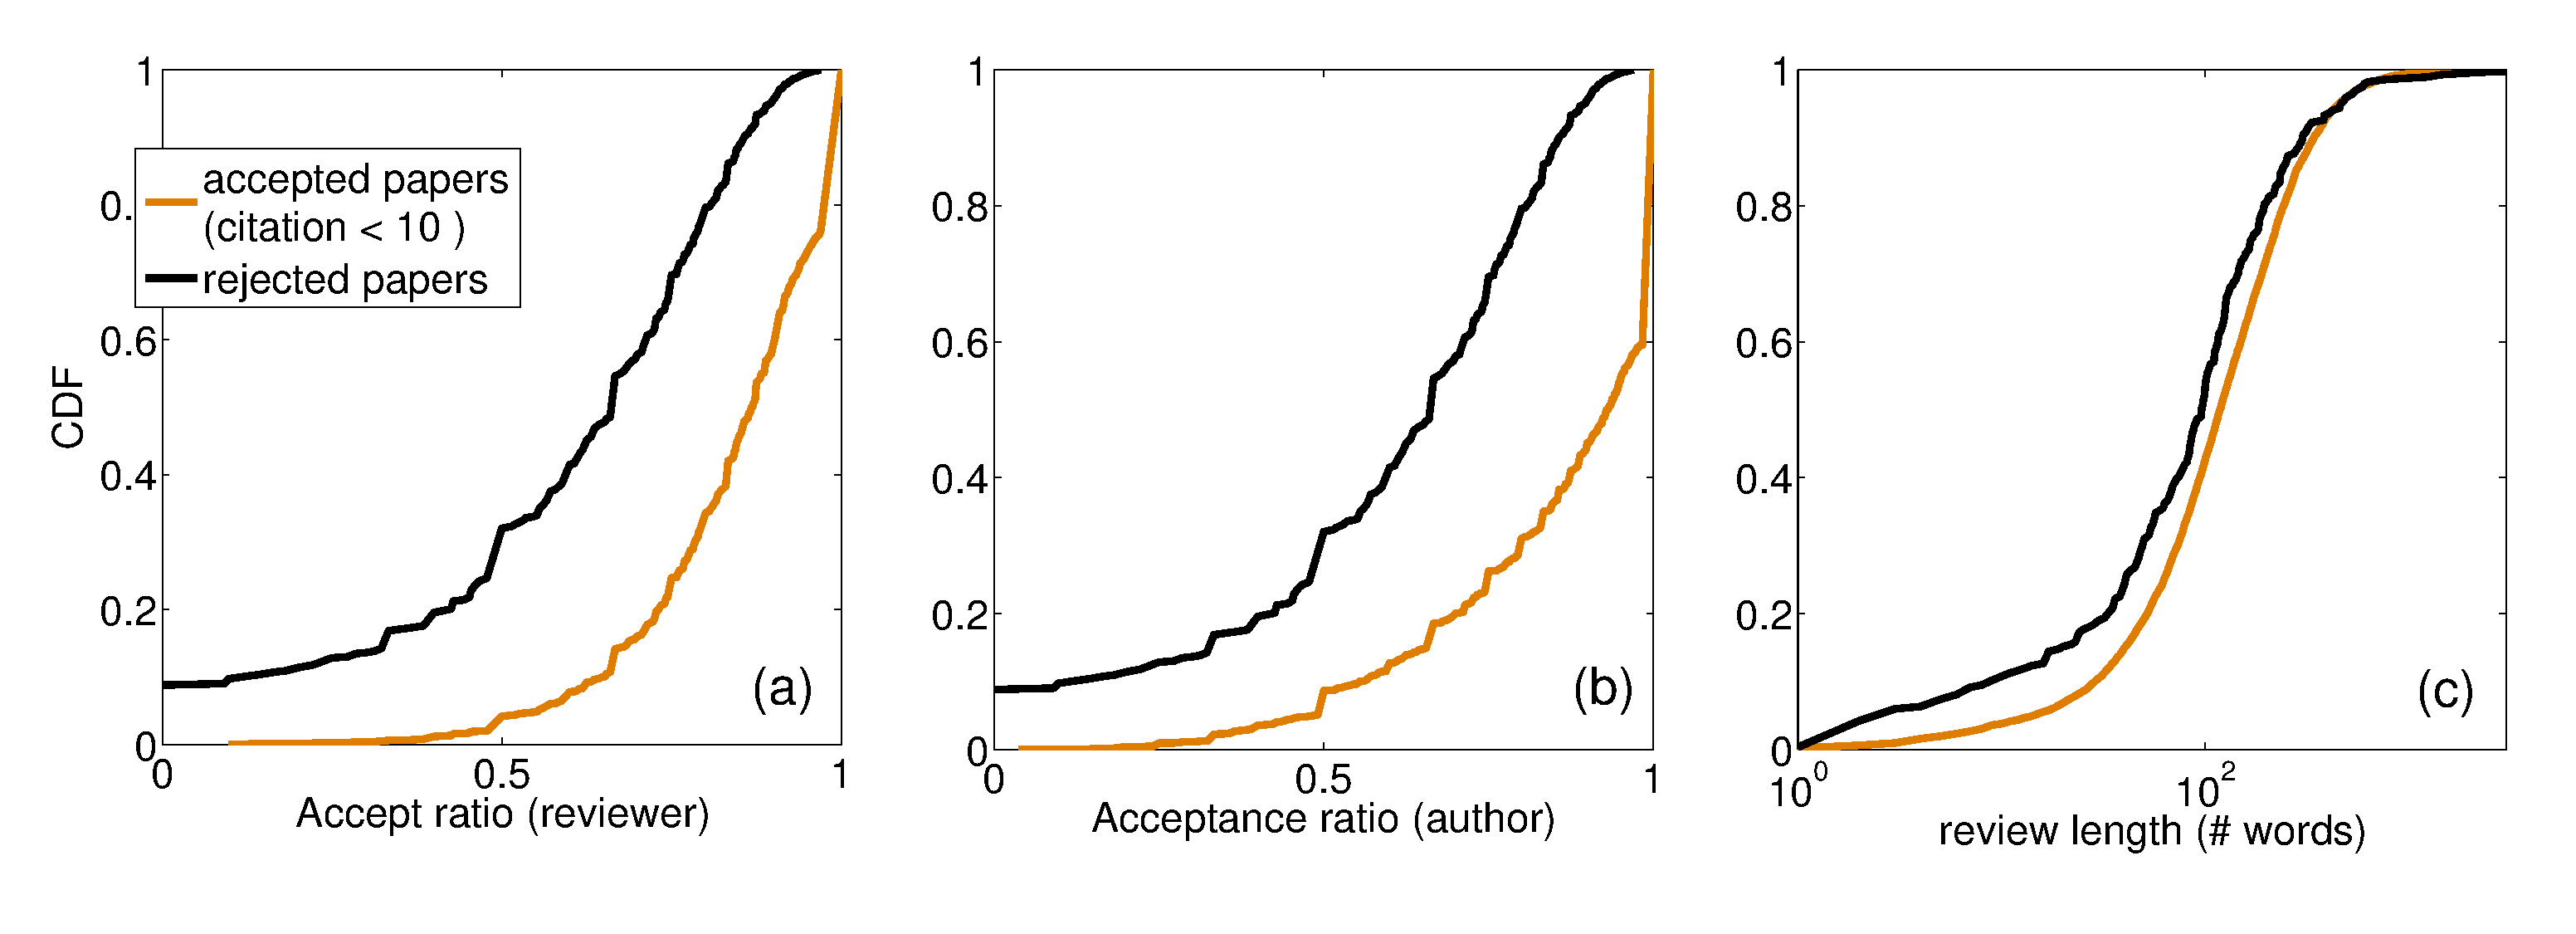
\includegraphics[scale=0.17]{./texfiles/Chapter_4/jcdl/figures/low_cited_accepted-eps-converted-to.pdf}
\caption{CDF of (a) accept ratio of reviewers, (b) acceptance ratio of authors (c) length of the review text (\# words) for rejected papers and low cited accepted papers.}
\label{fig11}
%\vspace{-1mm}
\end{figure}



\label{irregular_cases}

In this section we investigate in more detail the irregular cases, i.e., the highly cited rejected papers and the low cited accepted papers. Note that we only consider papers which were published before 2012 so that each paper gets at least three years of exposure to the scientific community for garnering citations.

\noindent{\em Highly cited rejected papers:} We previously observed that on average the accepted papers tend to be cited more often than the rejected ones. Nevertheless, we find several papers (call it the set $P$) which were rejected at JHEP but were able to acquire more citations after getting accepted elsewhere. We consider only those papers in $P$ that have at least 20 citations which is twice the average citation of the rejected papers.
Manually looking into some of the review text we observed that in several cases the reviewer found the topic of research to be interesting but out of JHEP's scope. On deeper investigation we found that acceptance ratio of the authors of these papers is lower than that of the authors of accepted papers (fig.~\ref{fig10}(a)) indicating that author's reputation might have played a role in the rejection. We further observe that the accept ratio of the reviewers, these papers were assigned to, to be significantly less than that of the accepted papers (fig.~\ref{fig10}(b)). This indicates that the papers got assigned to stricter reviewers and hence the rejection.

\noindent{\em Low cited accepted papers:} We now look into the complementary i.e., the papers which were accepted but failed to make impact on the scientific community and accrued very low citations (typically $< 10$). Ideally, these papers should have been rejected, hence we investigate how different these are in terms of author's acceptance ratio and reviewer's accept ratio. While the authors of these papers have higher acceptance ratio (fig.~\ref{fig11}(a)), they were also assigned to reviewers who are less strict (fig.~\ref{fig11}(b)). These observations indicate that either the contributing author's reputation might have played a role in their acceptance or were lucky to have been reviewed by lenient referees. Review report also seem to be sloppy in many cases with the reviewer not even mentioning the reason for acceptance. We also observe the length of the review report (in terms of the number of words) on average to be less than that of the rejected papers (fig.~\ref{fig11}(c)). 
%\medskip


\noindent
\section{Publisher's views}
\label{implication}
We further requested the JHEP journal administrators to survey our findings. The publishers pointed out the following observations to be of great significance -- 
(i) that reviewers excessively accepting/rejecting often fail to judge correctly the quality of the article, could be useful in assigning referees;
(ii) the number of review request does not necessarily improve the quality of the article. This observation could help in improving the efficiency of the peer-review process since both cost and time are involved for each round of review request; 
(iii) since only $10\%$ of the submissions were assigned to multiple reviewers and in most cases they failed to reach consensus, the publishers felt the need to investigate this issue more deeply by having frequent multiple assignments henceforth; 
(iv) the framework for predicting the long-term impact of the paper would be extremely helpful in assisting the editors in taking decisions. This might also aid in tracking the performance of the referees;
(v) that a significant fraction of authors have high acceptance rate at JHEP indicates a presence of at least a weak bias in the peer-review process and hence needs to be investigated;
\medskip



%\vspace{-3mm}

